\documentclass[xcolor=dvipsnames,12pt,aspectratio=169]{beamer}
\usecolortheme[named=violet]{structure} 

%\usetheme{umbc2} 
\usepackage{pgf}
%\usepackage[pdftex]{graphicx}
\usepackage{color}
\usepackage{amssymb,amsmath}
\usepackage[english]{babel}
\mode<presentation>

 \usepackage{multimedia}
\usefonttheme{structurebold}

%\useinnertheme{umbcboxes}

%\setbeamercolor{umbcboxes}{bg=violet!15,fg=black}  

\setbeamercovered{transparent}
\setbeamertemplate{navigation symbols}{}

%
%
% Adjustable parenthesis et al
%
\newcommand{\K}[1]{\left({#1}\right)}
\newcommand{\lp}{\left(}
\newcommand{\rp}{\right)}
\newcommand{\lb}{\left[}
\newcommand{\rb}{\right]}
\newcommand{\lc}{\left\{}
\newcommand{\rc}{\right\}}
\newcommand{\la}{\left\langle}
\newcommand{\ra}{\right\rangle}
\newcommand{\Dp}[3]{\langle #1,#2 \rangle_{#3}}
\newcommand{\cov}[2]{\langle #1\,#2 \rangle}

\newcommand{\half}{\mbox{$\frac{1}{2}$}} %

\newcommand{\U}{{\cal U}}
\newcommand{\C}{{\cal C}}
\newcommand{\X}{{\cal X}}
\newcommand{\Y}{{\cal Y}}

\newcommand {\ared} {{\rm ared}}
\newcommand {\pred} {{\rm pred}}
\newcommand {\rpred} {{\rm rpred}}

\newcommand{\sn}{s^{\sf n}}  % Normal component
\newcommand{\st}{s^{\sf t}}  % Tangential component
\newcommand{\rt}{r^{\sf t}}  % Tangential component
\newcommand{\stepy}{{s_y}}  % step in y--component
\newcommand{\stepu}{{s_u}}  % step in u--component

%
\newcommand{\veps}{{\varepsilon}} 
% Bolds and scripts
%
\newcommand{\CG}{\ensuremath{\mathcal{G}} }
\newcommand{\CQ}{\ensuremath{\mathcal{Q}} } %
\newcommand{\CR}{\ensuremath{\mathcal{R}} } %
\newcommand{\CW}{\ensuremath{\mathcal{W}} } %
\newcommand{\CX}{\ensuremath{\mathcal{X}} } %
\newcommand{\CZ}{\ensuremath{\mathcal{Z}} } %
\newcommand{\CU}{\ensuremath{\mathcal U} }
\newcommand{\CC}{\ensuremath{\mathcal C} }
\newcommand{\CD}{\ensuremath{\mathcal D} }
\newcommand{\BA}{\ensuremath{\mathbf{A}} } %
\newcommand{\BB}{\ensuremath{\mathbf{B}} } %
\newcommand{\BC}{\ensuremath{\mathbf{C}} } %
\newcommand{\BhC}{\ensuremath{\widehat{\mathbf{C}}} } %
\newcommand{\BD}{\ensuremath{\mathbf{D}} } %
\newcommand{\BE}{\ensuremath{\mathbf{E}} } %
\newcommand{\BF}{\ensuremath{\mathbf{F}} } %
\newcommand{\BG}{\ensuremath{\mathbf{G}} } %
\newcommand{\BH}{\ensuremath{\mathbf{H}} } %
\newcommand{\BK}{\ensuremath{\mathbf{K}} } %
\newcommand{\BL}{\ensuremath{\mathbf{L}} } %
\newcommand{\BM}{\ensuremath{\mathbf{M}} } %
\newcommand{\BN}{\ensuremath{\mathbf{N}} } %
\newcommand{\BP}{\ensuremath{\mathbf{P}} } %
\newcommand{\BQ}{\ensuremath{\mathbf{Q}} } %
\newcommand{\BR}{\ensuremath{\mathbf{R}} } %
\newcommand{\BU}{\ensuremath{\mathbf{U}} } %
\newcommand{\BW}{\ensuremath{\mathbf{W}} } %
\newcommand{\BX}{\ensuremath{\mathbf{X}} } %
\newcommand{\BY}{\ensuremath{\mathbf{Y}} } %
\newcommand{\BZ}{\ensuremath{\mathbf{Z}} } %
\newcommand{\ba}{\ensuremath{\mathbf{a}}}
\newcommand{\bb}{\ensuremath{\mathbf{b}}}
\newcommand{\bc}{\ensuremath{\mathbf{c}}}
\newcommand{\be}{\ensuremath{\mathbf{e}}}
\newcommand{\bg}{\ensuremath{\mathbf{g}}} %
\newcommand{\bh}{\ensuremath{\mathbf{h}}} %
\newcommand{\bk}{\ensuremath{\mathbf{k}}} %
\newcommand{\bn}{\ensuremath{\mathbf{n}}} %
\newcommand{\bp}{\ensuremath{\mathbf{p}}} %
\newcommand{\bq}{\ensuremath{\mathbf{q}}}
\newcommand{\br}{\ensuremath{\mathbf{r}}} %
\newcommand{\bs}{\ensuremath{\mathbf{s}}} %
\newcommand{\bt}{\ensuremath{\mathbf{t}}} %
\newcommand{\bu}{\ensuremath{\mathbf{u}}} %
\newcommand{\bv}{\ensuremath{\mathbf{v}}} %
\newcommand{\bdv}{\ensuremath{\mathbf{\delta v}}} %
\newcommand{\bw}{\ensuremath{\mathbf{w}}} %
\newcommand{\bd}{\ensuremath{\mathbf{d}}} %
\newcommand{\bx}{\ensuremath{\mathbf{x}}} %
\newcommand{\by}{\ensuremath{\mathbf{y}}} %
\newcommand{\obx}{\ensuremath{\overline{\mathbf{x}}}} %
\newcommand{\oby}{\ensuremath{\overline{\mathbf{y}}}} %
\newcommand{\obz}{\ensuremath{\overline{\mathbf{z}}}} %
\newcommand{\obw}{\ensuremath{\overline{\mathbf{w}}}} %
\newcommand{\bz}{\ensuremath{\mathbf{z}}} %
\newcommand{\blambda}{\mbox{\boldmath $\lambda$}}
\newcommand{\bdelta}{\mbox{\boldmath $\delta$}}
\newcommand{\bxi}{\mbox{\boldmath{$\xi$}}}
\newcommand{\bfeta}{\mbox{\boldmath $\eta$}}
\newcommand{\bkappa}{\mbox{\boldmath $\kappa$}}
\newcommand{\bmu}{\mbox{\boldmath $\mu$}}
\newcommand{\brho}{\mbox{\boldmath $\rho$}}
\newcommand{\bsigma}{\mbox{\boldmath $\sigma$}}
\newcommand{\sbxi}{\mbox{\scriptsize \boldmath{$\xi$}}}
\newcommand{\sbfeta}{\mbox{\scriptsize \boldmath $\eta$}}
\newcommand{\teta}{\mbox{\tiny \boldmath $\eta$}}
\newcommand{\txi}{\mbox{\tiny \boldmath{$\xi$}}}
\newcommand{\bLambda}{\mbox{\boldmath $\Lambda$}}
\newcommand{\bDelta}{\mbox{\boldmath $\Delta$}}
\newcommand{\bzero}{\mbox{\boldmath $0$}}
\newcommand{\bone}{\mbox{\boldmath $1$}}
\newcommand{\sDelta}{\mbox{\small $\Delta$}}
\newcommand{\tDelta}{\mbox{\tiny $\Delta$}}

\newcommand{\pd}[2]{\frac{\partial #1}{\partial #2}}
\newcommand{\ppd}[3]{\frac{\partial^{#3} #1}{\partial {#2}^{#3}}}
\newcommand{\pdsec}[3]{\frac{\partial^2 #1}{\partial #2\partial #3}}

\def\frechet{Fr\'echet\ }
%\newcommand{\real}{\mathbb{R}}
\newcommand{\real} {I\!\!R}
\newcommand{\nat} {{I\!\!N}}
\newcommand{\compl} {C\!\!\!\!I\;}
%
\def\Pr{\sf Pr}
\def\Re{\sf Re}
\def\M{{\sf M}}
\def\d{\delta}
\newcommand{\deq}{\raisebox{0pt}[1ex][0pt]{$\stackrel{\scriptscriptstyle{\rm def}}{{}={}}$}}
\newcommand{\dif}{{\mathrm d}}

\newcommand{\eref}[1]{\mbox{\rm(\ref{#1})}}
\newcommand{\tref}[1]{\mbox{\rm\ref{#1}}}


%\newenvironment{proof}{\noindent {\bf Proof:} }{\hfill $\Box$ \\[2ex] }

\newcommand{\myint}[1]{\int_0^T \dif t~{#1}}
\newcommand{\myintt}[1]{\int_0^1 \dif s~{#1}}
\newcommand{\dint}[1]{\int\limits_{#1}\!\!\!\int}

\newcommand{\waveop}[1]{c^{-2}{#1}_{tt}-\Delta{#1}}
\newcommand{\redwaveop}[1]{\Delta{#1}+k^2n^2{#1}}

\newcommand{\D}{\displaystyle}
%\allowdisplaybreaks
%

\setlength{\parskip}{2ex}   % place a blank line between paragraphs
\def\Logo{\@ifnextchar(\beamer@Logo\logo}
\def\beamer@Logo(#1,#2){\logo}

\AtBeginSection[]{
{\setbeamertemplate{logo}{}
 \begin{frame}<beamer>
    \frametitle{Agenda}
    \tableofcontents[currentsection]
  \end{frame}
}
}
% Images
% Macros
\newcommand{\peq}{\,+\hspace{-0.15cm}=}
\newcommand{\bm}{\bar{m}}
\newcommand{\dm}{\delta m}
\newcommand{\dom}{\delta \bar{m}}
\newcommand{\doma}{\delta \bar{m}_{\alpha}}
\newcommand{\om}{\bar{m}}
\newcommand{\bH}{{\bf H}}
\newcommand{\bR}{{\bf R}}
\newcommand{\bcF}{{\bar{\cal F}}}
\newcommand{\cF}{{\cal F}}
\newcommand{\oF}{\bar{F}}
\newcommand{\odF}{\bar{F}^{\dagger}}
\newcommand{\oS}{\bar{S}}
\newcommand{\oM}{\bar{M}}
\newcommand{\Ja}{J_{\alpha}}
\newcommand{\Na}{N_{\alpha}}
\newcommand{\dd}{\delta d}
\newcommand{\ddl}{\delta d_{\alpha}}
\title[]{Accelerating Acoustic Least Squares Migration}
\author[]{Raanan Dafni \& William W. Symes}
\institute[]{The Rice Inversion Project\\Computational and Applied Mathematics\\Rice University}
\date{SEG Anaheim 2018}

\begin{document}
\frame{
\titlepage
}

\begin{frame}\frametitle{Overview}

Takeaway:  {\color{blue}T}rue {\color{blue}A}mplitude {\color{blue}M}igration = transpose of Born modeling w.r.t. {\em weighted dot products} $\Rightarrow$ rapidly convergent {\color{blue}P}reconditioned {\color{blue}C}onjugate {\color{blue}G}radient iteration for {\color{blue}L}east {\color{blue}S}quares {\color{blue}M}igration

Agenda:
\begin{itemize}
\item Feasible TAM computation 
\item How to formulate accelerated LSM via PCG
\item Necessary conditions for successful PCG
\end{itemize}
\end{frame}

\section{True Amplitude Migration}

\begin{frame}
Varieties of TAM:

\begin{itemize}
\item Generalized Radon Transform / ray-Born / Kirchhoff inversion: Beylkin 85, Bleistein 87,....
\item Scaling methods: Claerbout \& Nichols 94, Nammour \& S. 09, ...
\item {\color{blue}Wave Equation TAM}: Zhang, Bleistein et al. 03, 05,,..., ten Kroode 12, Hou \& S. 15, 17
\end{itemize}

Aim of Wave Equation TAM: achieve inversion similar to GRT with {\em no ray tracing} - only wave equation solves
\end{frame}

\begin{frame}
Acoustic wave system, isotropic point source - bulk modulus = $\kappa(\bx)$, density = $\rho(\bx)$, $w(t)$ = source pulse, $\bx_s$ = source position: pressure = $p(\bx,t;\bx_s)$, particle velocity = $\bv(\bx,t;\bx_s)$ (``source'' fields) satisfy
\[
\rho \frac{\partial \bv}{\partial t} = - \nabla p,\,\,
\frac{1}{\kappa}\frac{\partial p}{\partial t} = - \nabla \cdot \bv + w(t)\delta(\bx-\bx_s)
\]
\[
p, \bv = 0, t<<0
\]

Born system for perturbations $\delta \kappa$, {\color{blue} $\delta \rho = 0$}, $\delta p$, $\delta \bv$:
\[
\rho \frac{\partial \delta \bv}{\partial t} = - \nabla \delta p,\,\,
\frac{1}{\kappa}\frac{\partial \delta p}{\partial t} = - \nabla \cdot \delta \bv + \frac{\delta \kappa}{\kappa^2} \frac{\partial p}{\partial t} 
\]
\[
\delta p, \delta \bv = 0, t << 0
\]

Born modeling op: $F_w \delta \kappa (\bx_r,t; \bx_s) = \delta p(\bx_r,t;\bx_s) $ 
\end{frame}

\begin{frame}
\vspace{-0.5cm}
\begin{center}
%\includegraphics[height=5cm]{Fig/coarse1bulk}\includegraphics[height=5cm]{Fig/equals}
%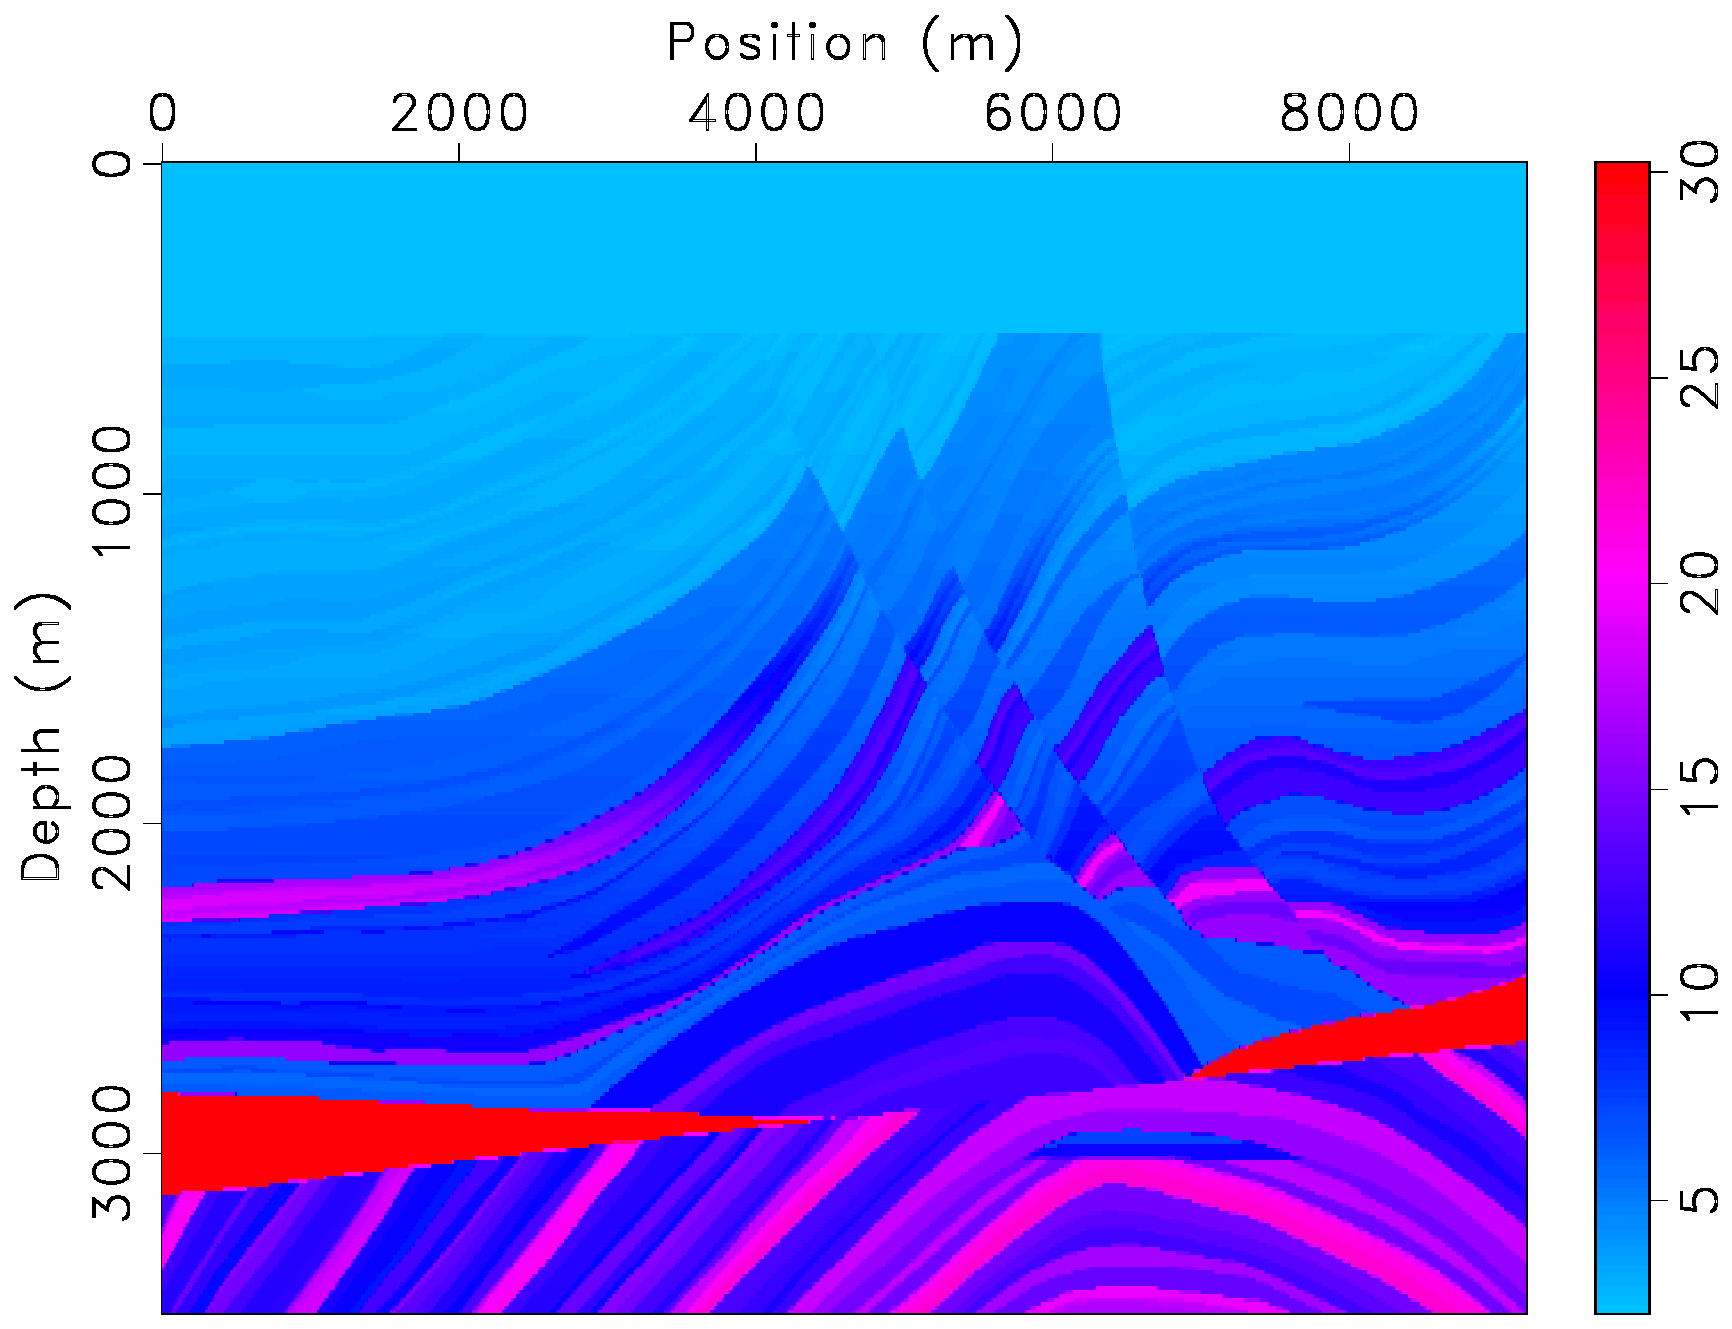
\includegraphics[height=5cm]{Fig/fine1bulk}\includegraphics[height=5cm]{Fig/equals}
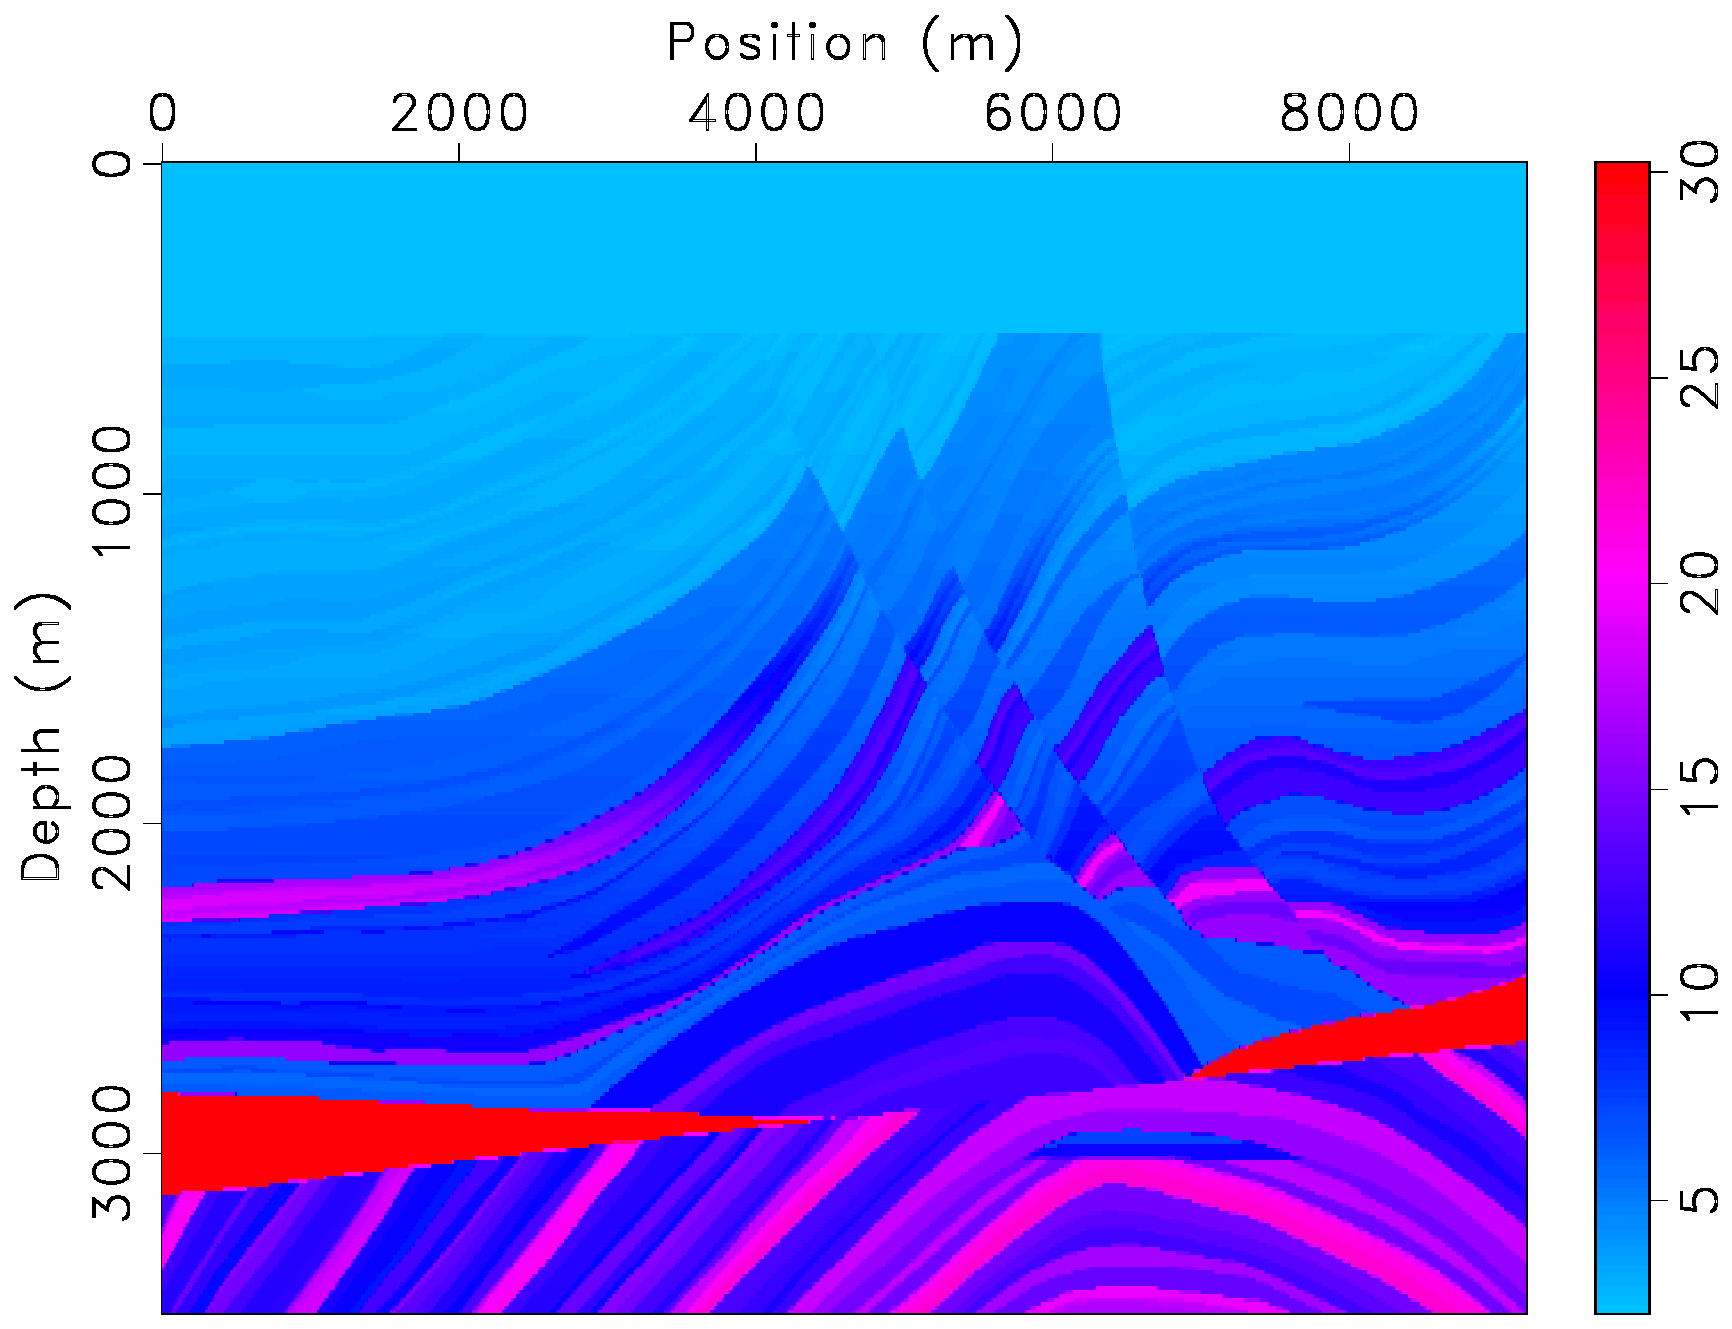
\includegraphics[height=5.5cm]{Fig/fine1bulk}\\
$\kappa_0$ = Marmousi bulk modulus = $\kappa + \delta \kappa$
\end{center}
\vspace{-0.5cm}
\end{frame}

\begin{frame}
\vspace{-0.5cm}
\begin{center}
%\includegraphics[height=5cm]{Fig/coarse1bulkbig}\includegraphics[height=5cm]{Fig/plus}
%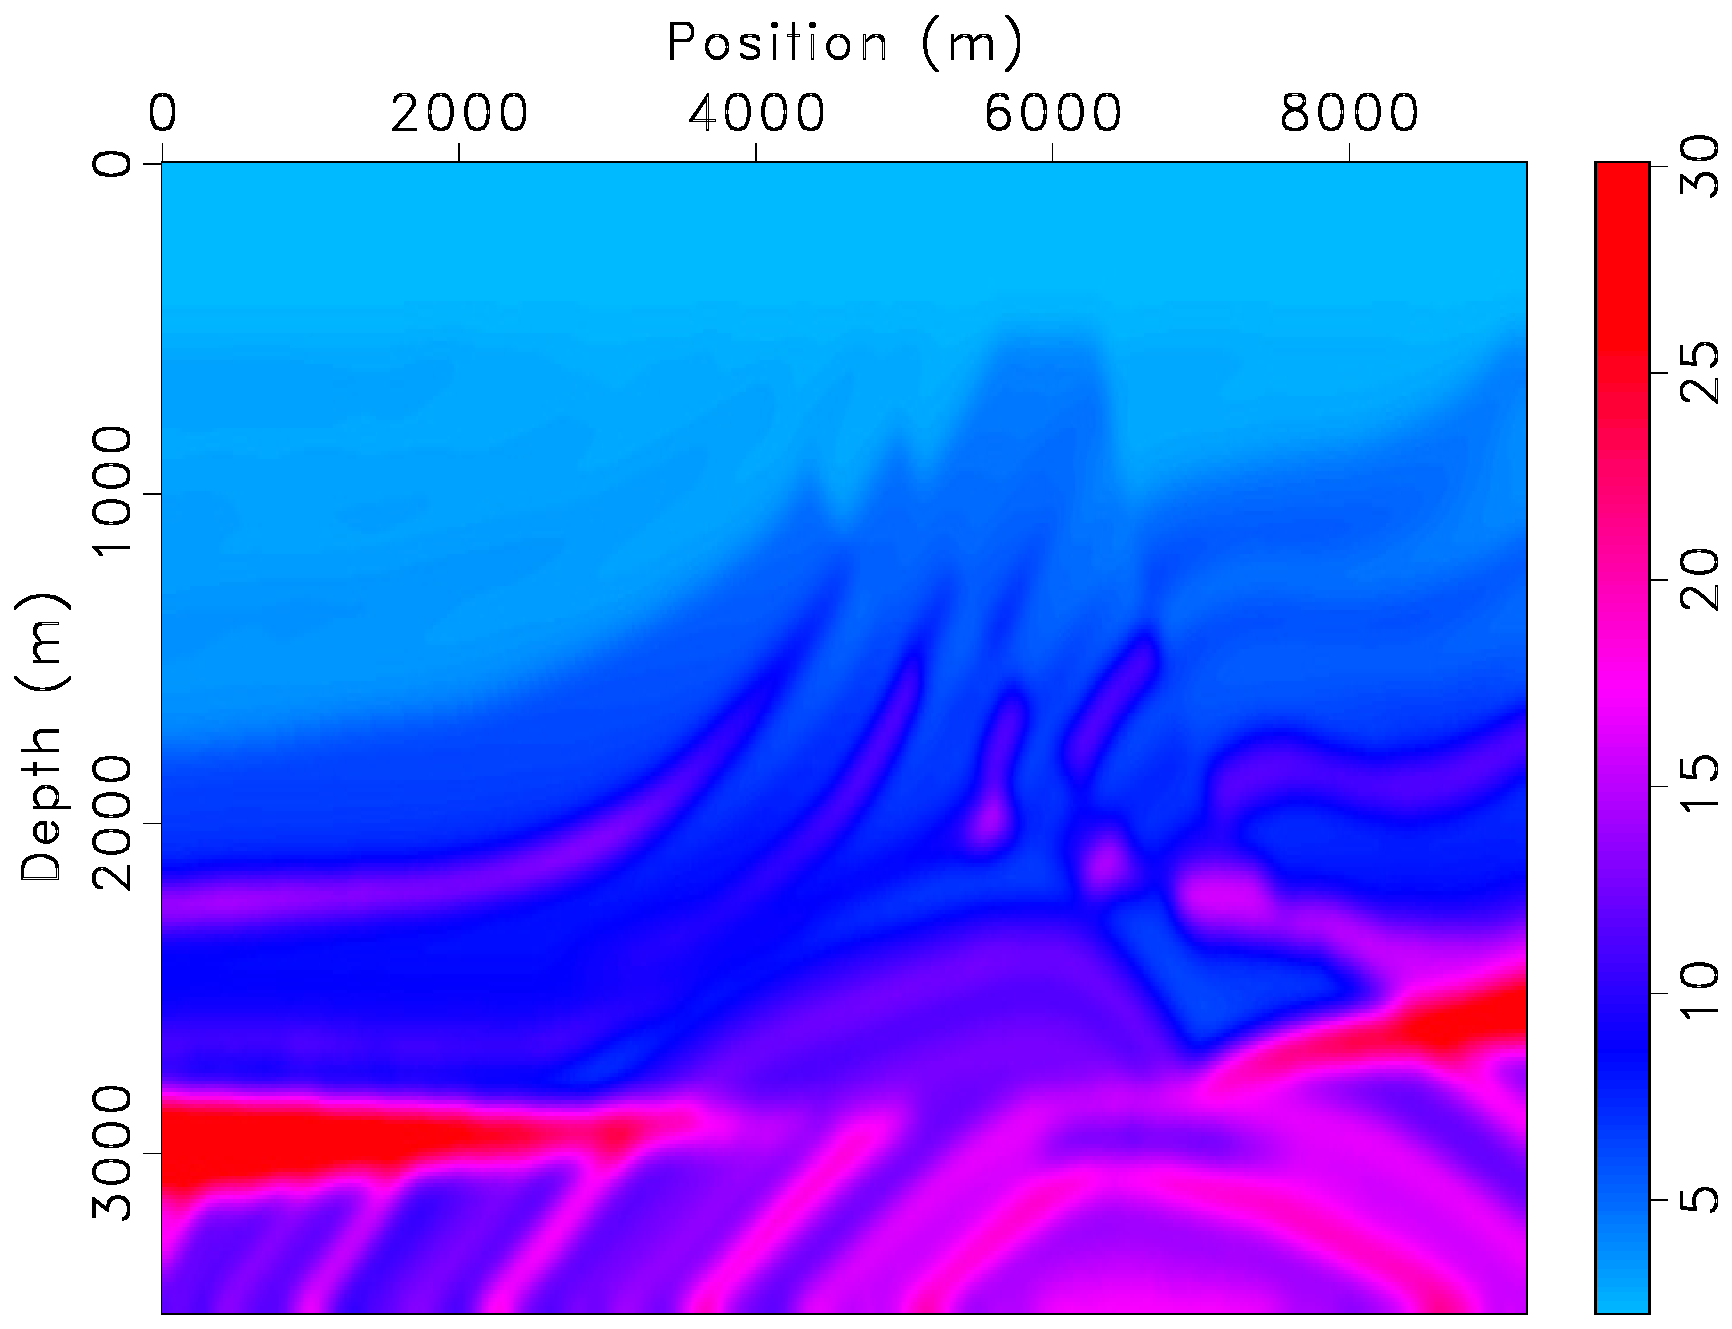
\includegraphics[height=5cm]{Fig/fine1bulkbig}\includegraphics[height=5cm]{Fig/plus}
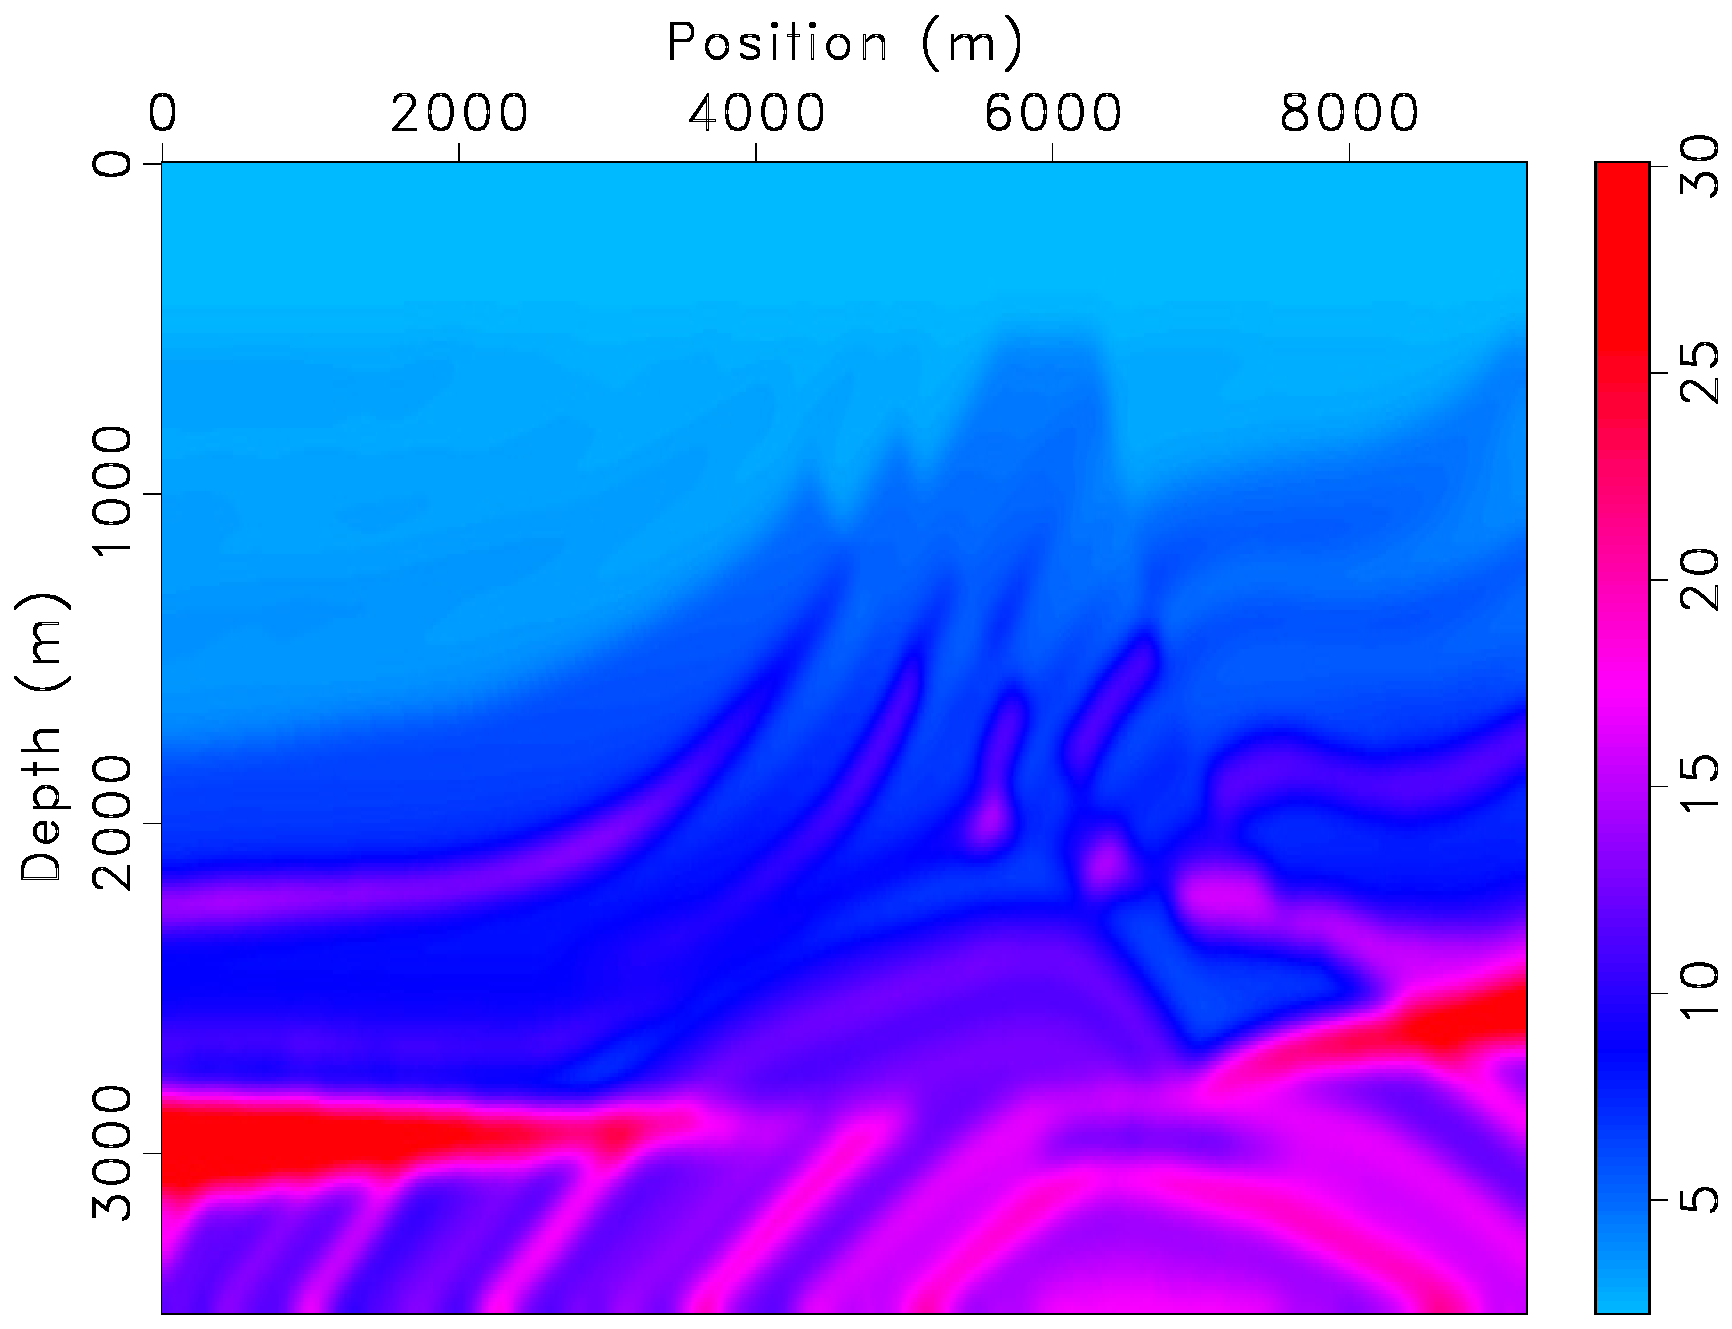
\includegraphics[height=5.5cm]{Fig/fine1bulkbig}\\
$\kappa$ = background = spatial moving average 
\end{center}
\vspace{-0.5cm}
\end{frame}

\begin{frame}
\vspace{-0.5 cm}
\begin{center}
%\includegraphics[height=5.5cm]{Fig/coarse1dbulk}\\
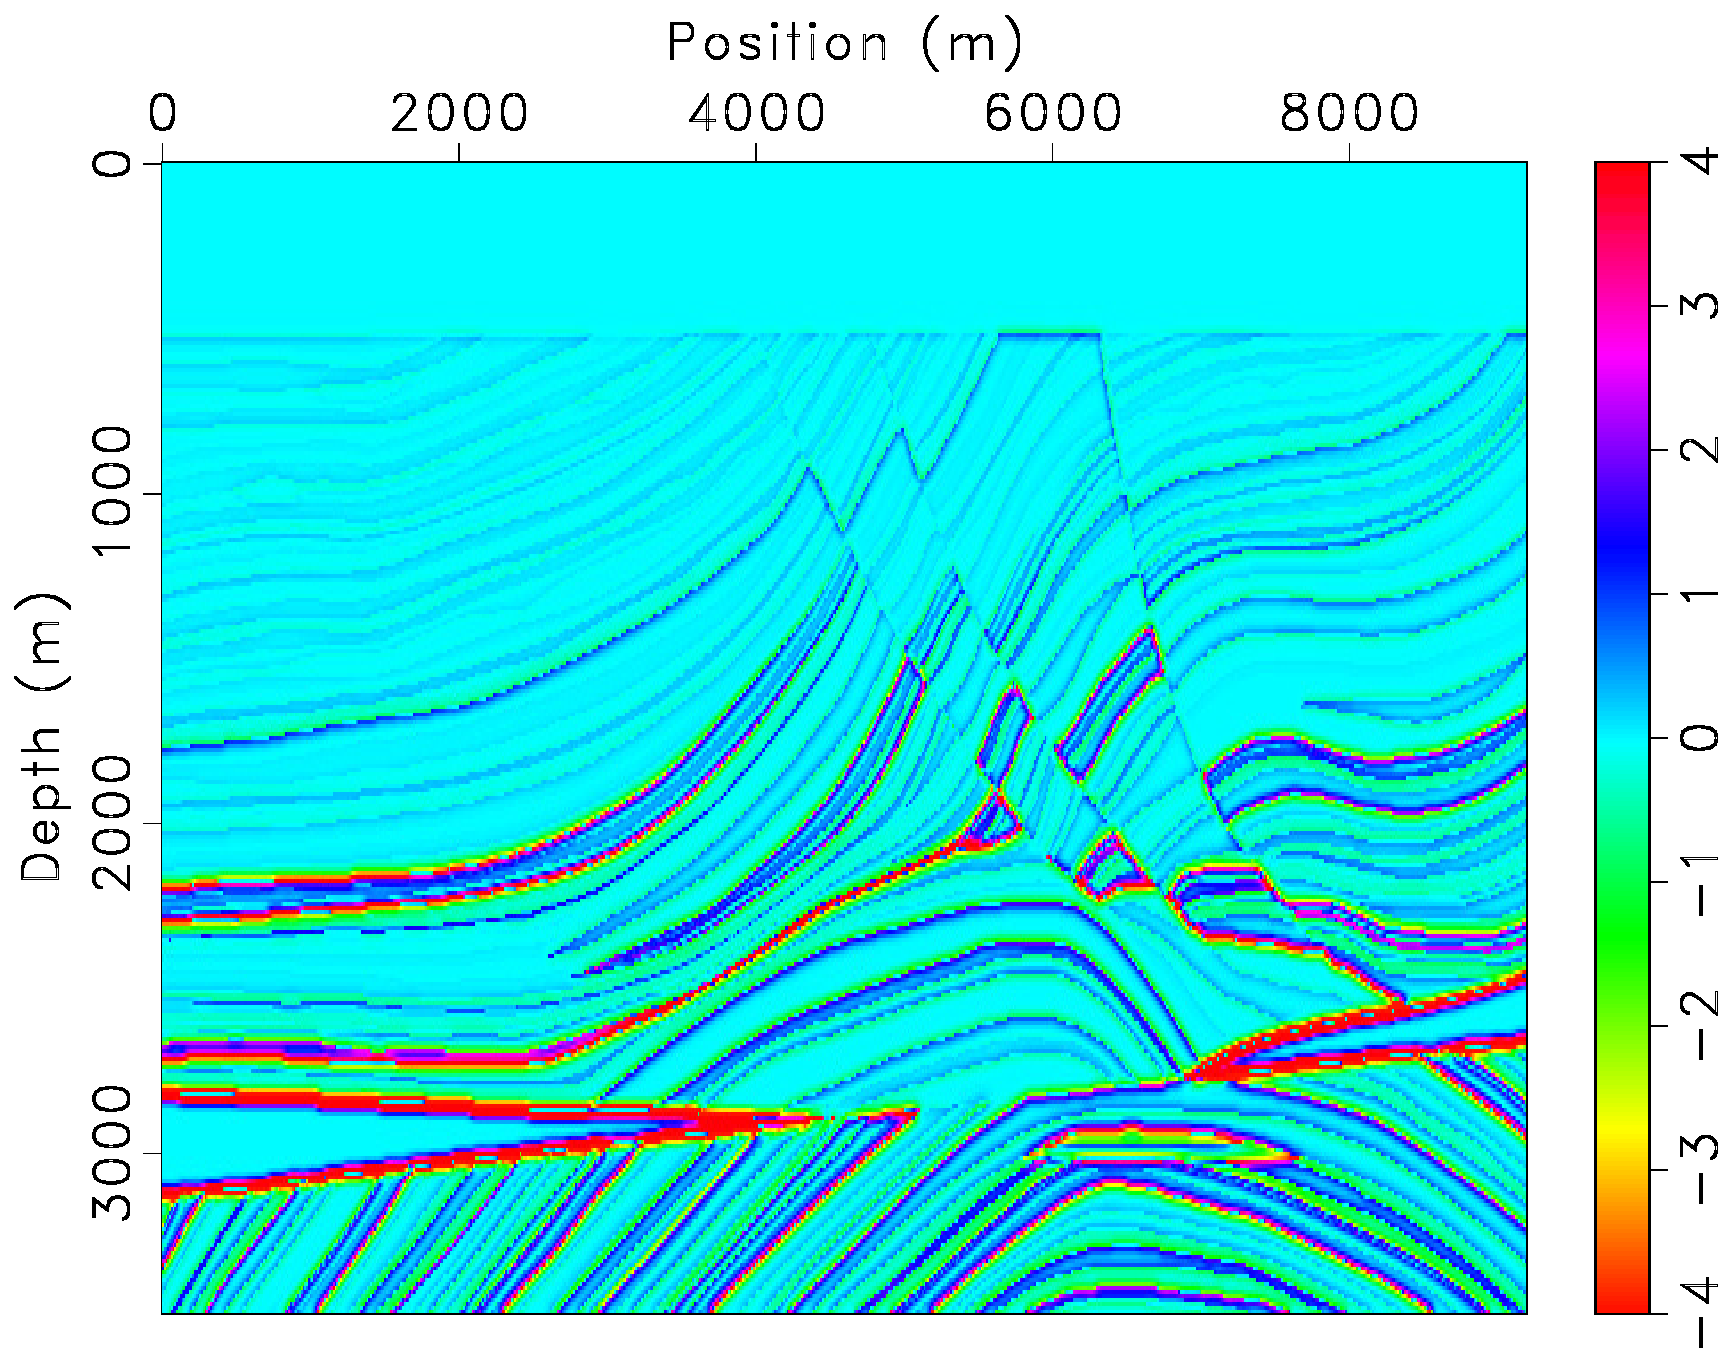
\includegraphics[height=5.5cm]{Fig/fine1dbulk}\\
$\delta \kappa$ = model perturbation = $\kappa_0-\kappa$
\end{center}
\end{frame}

\begin{frame}
%\vspace{-1.0cm}
\begin{center}
%\includegraphics[height=6cm]{Fig/coarse1bornr45}
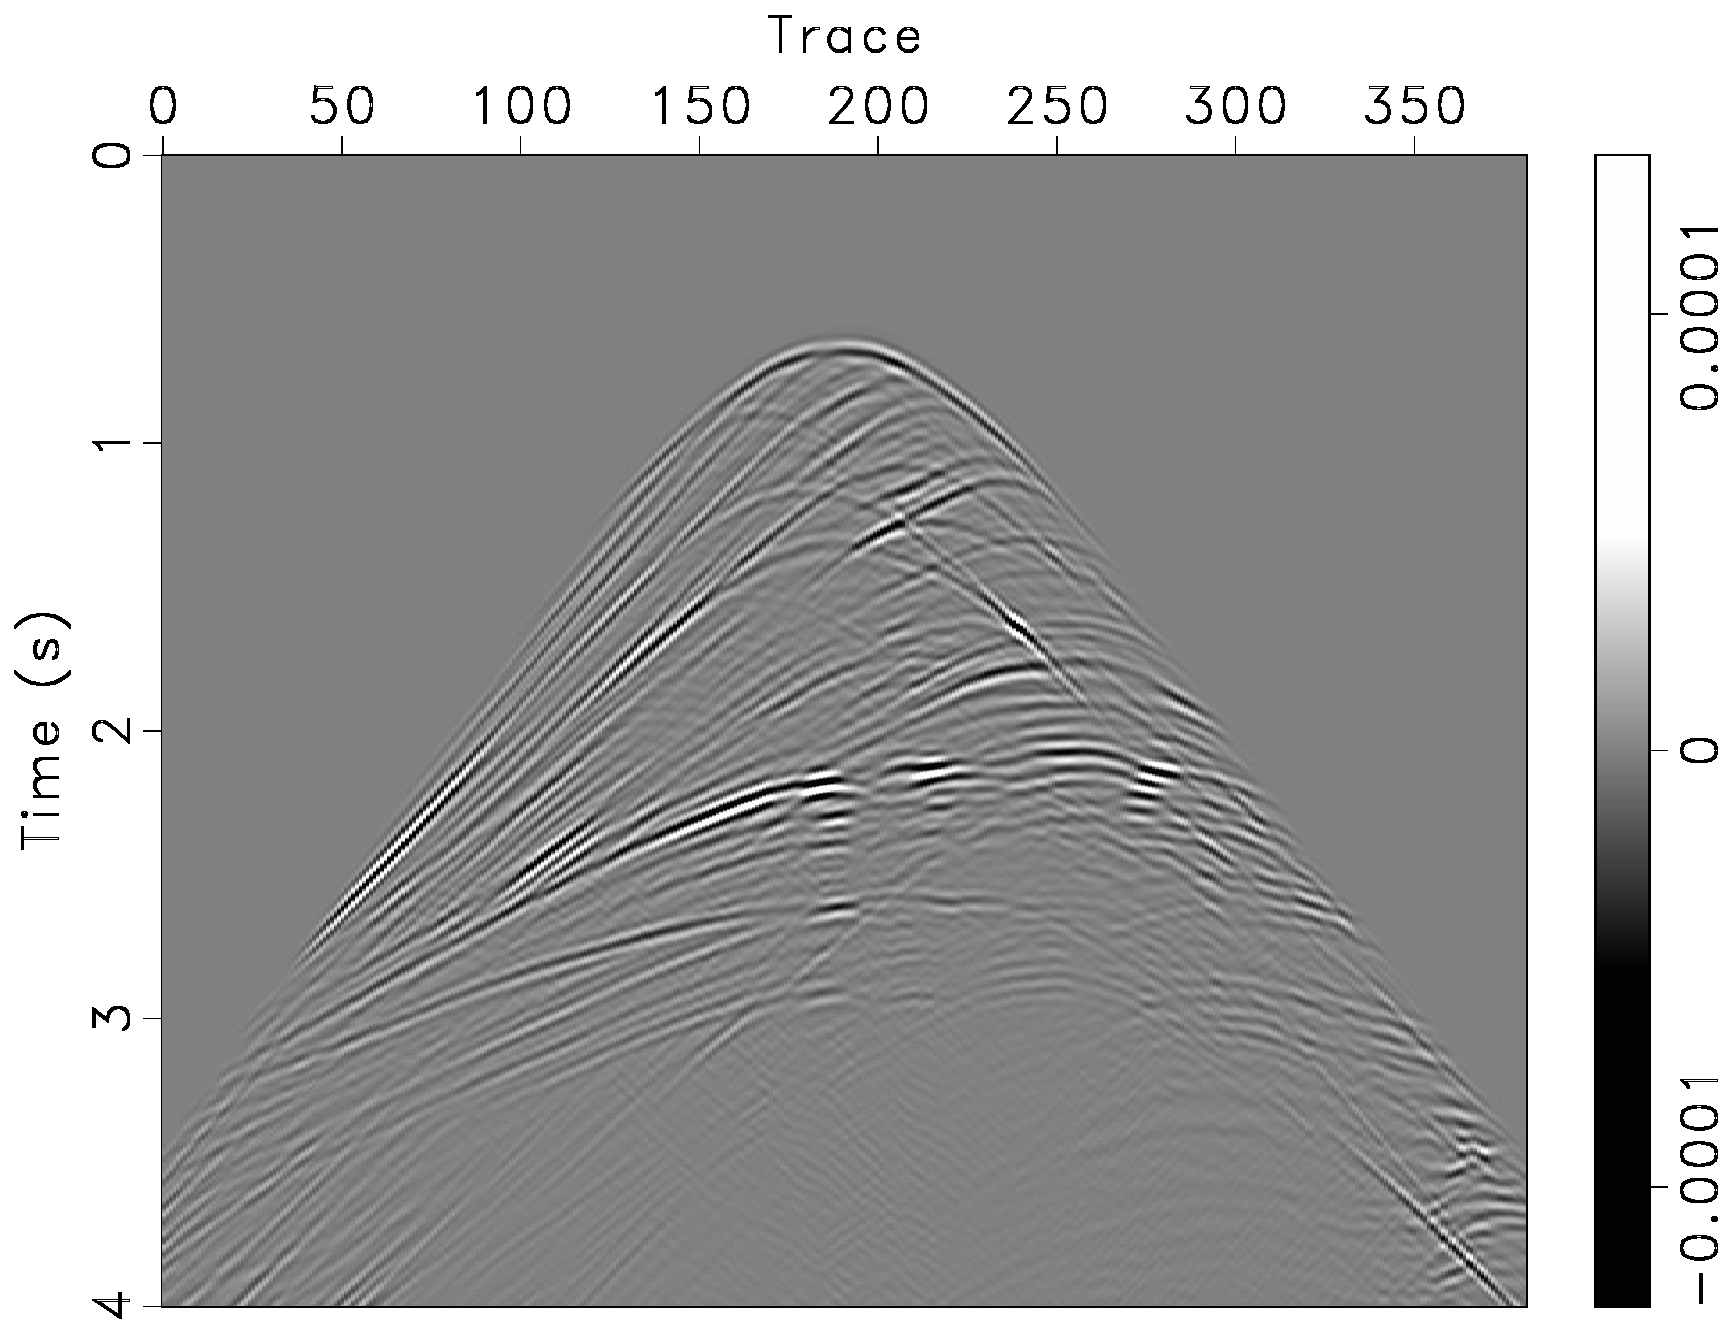
\includegraphics[height=6cm]{Fig/fine1bornr90}\\
$\delta d = F_w\delta \kappa$ = First order predicted (linearized,
``Born'') free surface shot 90 \\(180 shots @ 48 m, 361 recvrs @ 24 m), $z_s=z_r=12$ m, $w = H * $ [2.5, 5, 25, 30] Hz trapezoidal bandpass
\end{center}
\end{frame}

\begin{frame}
Reverse Time Migration = transpose of Born modeling

RTM of perturbation data $\delta d(\bx_r,t;\bx_s)$:

- compute adjoint (``receiver'') fields $q(\bx,t;\bx_s), \bw(\bx,t;\bx_s)$
\[
\rho \frac{\partial \bw}{\partial t} = - \nabla q,\,\,
\frac{1}{\kappa}\frac{\partial q}{\partial t} = - \nabla \cdot \bw + \sum_{\bx_r} d(\bx_r,t;\bx_s) \delta(\bx-\bx_r)
\]
\[
q, \bw = 0, t >>0
\]

- cross-correlate with zero lag, sum over sources:
\[
F_w^T\delta d(\bx) = -\frac{1}{\kappa(\bx)^2}\sum_{\bx_s} \int\,dt\,\frac{\partial p}{\partial t}(\bx,t;\bx_s)q(\bx,t:\bx_s) 
\]
\end{frame}

\begin{frame}
\vspace{-1.0cm}
\begin{center}
%\includegraphics[height=7cm]{Fig/coarse1mbulk}\\
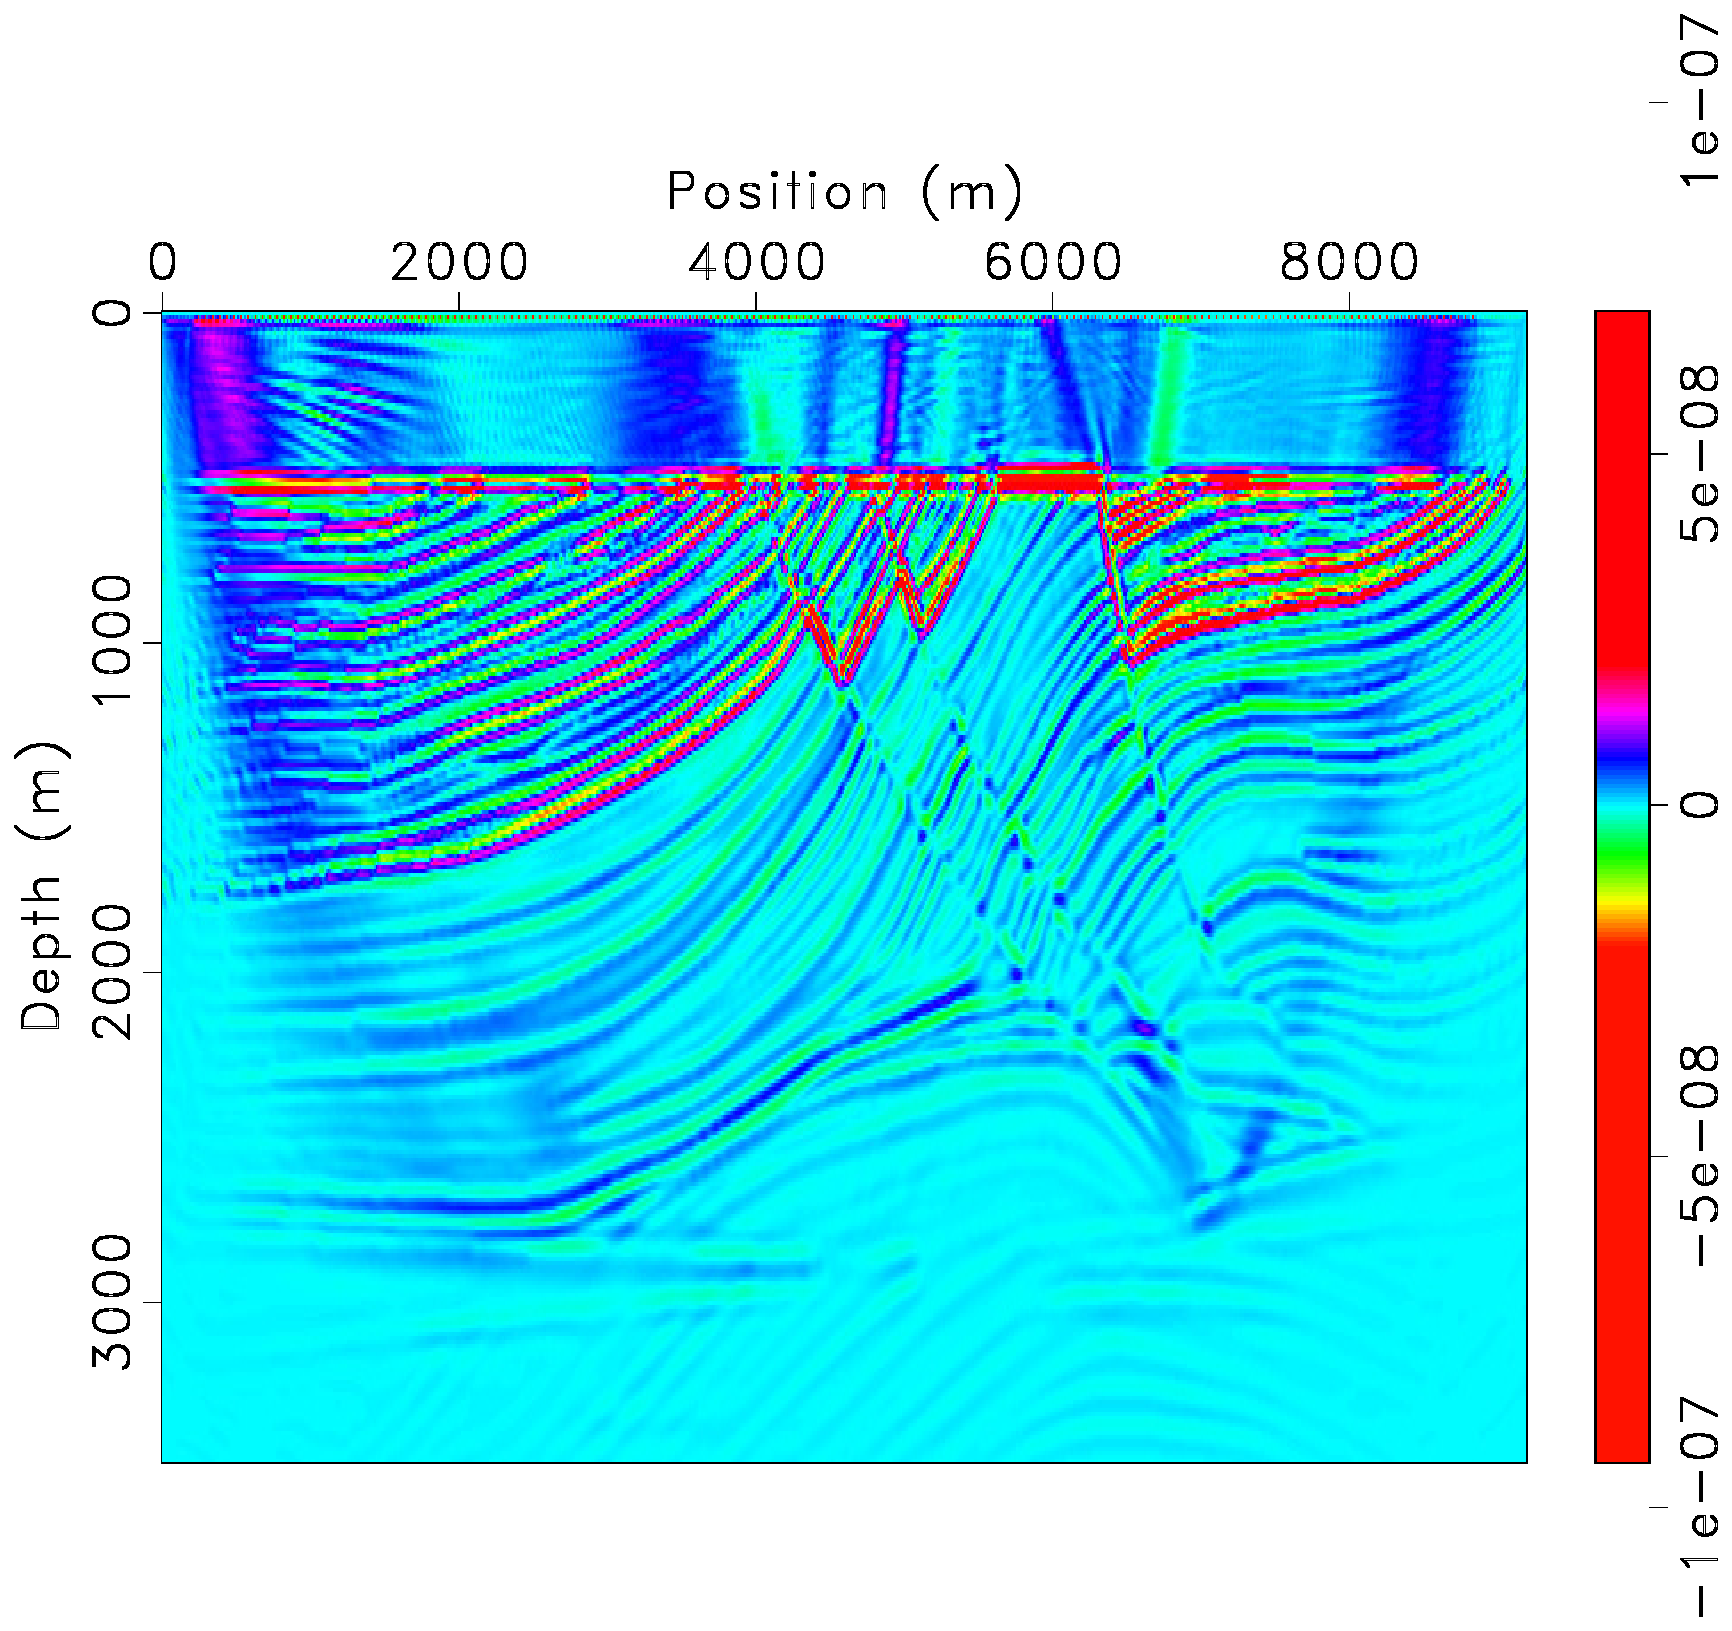
\includegraphics[height=7cm]{Fig/fine1mbulk}\\
$F_w^T\delta d$ = RTM image of $\delta \kappa$  
\end{center}
\end{frame}

\begin{frame}
\vspace{-0.7cm}
\begin{center}
%\includegraphics[height=5.1cm]{Fig/coarse1dbulk}\\
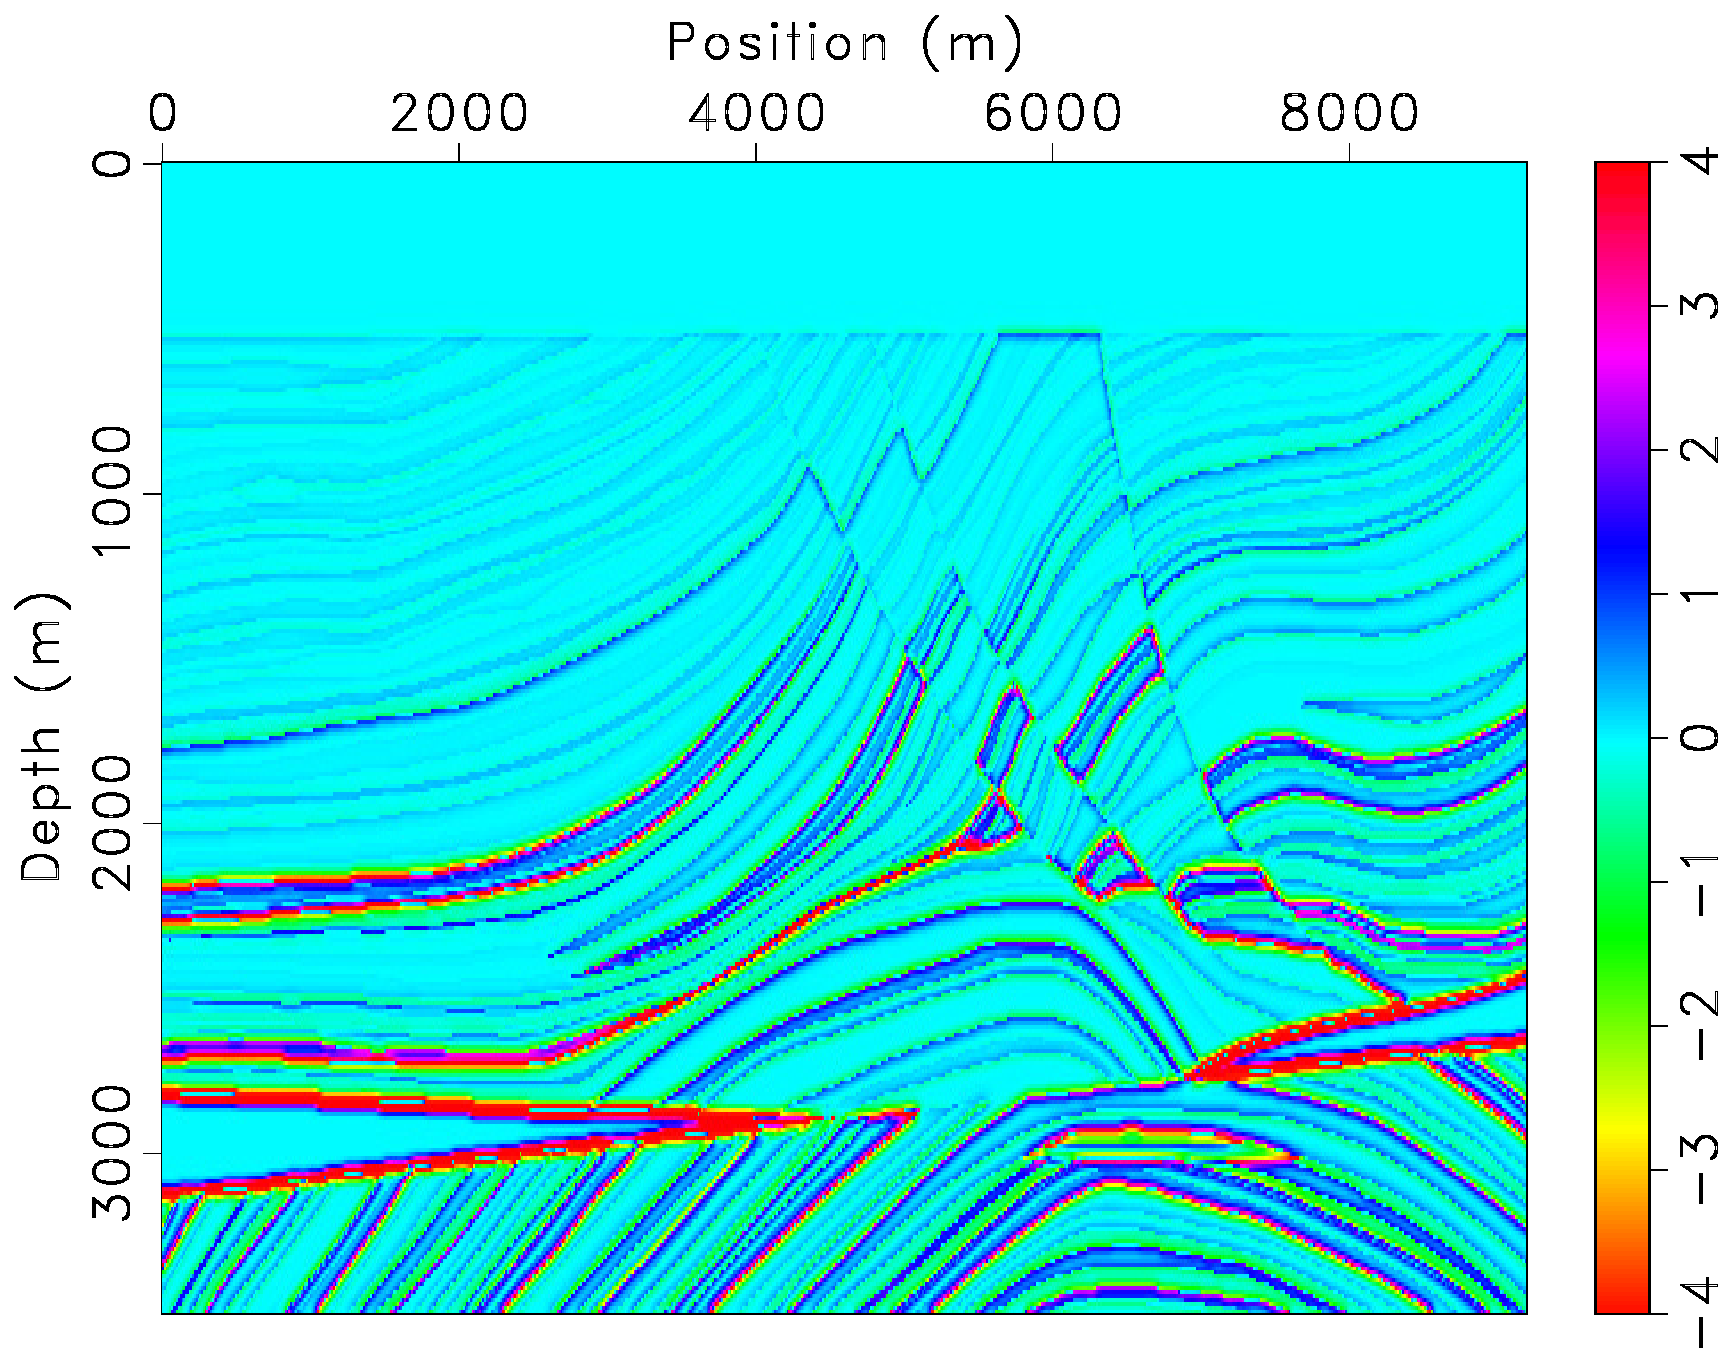
\includegraphics[height=5.8cm]{Fig/fine1dbulk}\\
$\delta \kappa$ = model perturbation
\end{center}
\end{frame}

\begin{frame}
Observations:

\begin{itemize}
\item +: reflector positions correct (correct velocity)
\item -: low spatial frequency noise (diving waves in source fields)
\item -: {\color{blue} wrong reflector amplitudes - relative and absolute errors}
\end{itemize}

\end{frame}


\begin{frame}
Asymptotic analysis
(Beylkin 85, Bleistein 87, Rakesh 88, Beylkin \& Burridge 89,...) - $w(t)=H(t)$ (practically: integrated bandpass filter), drop from notation:

\[
(I_tF)^TI_tF\delta \kappa(\bx) \approx \int d{\bf k} e^{i {\bf k}\cdot \bx} \frac{(...)}{\cos \theta_r \cos \theta_s} \delta \hat{\kappa}({\bf k})
\]
\begin{itemize}
\item $I_t$ = indef t-integral (Heaviside filter)
\item $\cos \theta_{s,r}$ = wave/ray angle of incidence at source, receiver
\item ``(...)'' = explicit filters,  functions of $\kappa_0(\bx),\rho(\bx)$
\end{itemize}
\end{frame}

\begin{frame}
Get rid of $\cos \theta_{s,r}$ by applying $D_{z_{s,r}}$ 

Get rid of filters, functions by applying inverse filters, reciprocals

$\Rightarrow$  true/preserved amplitude migration operator $(I_tF)^{\dagger}$ (Zhang \& Bleistein 03, 05,...,ten Kroode 12,...) Hou \& S. 15, 17: factorization
\[
(I_tF)^{\dagger} = W_m^{-1} (I_tF)^T W_d, 
\]
$W_m, W_d$ simple explicit filters: $W_d =  -|f|^{-3} D_{z_s} D_{z_r},\, W_m^{-1} = 32 \rho^{-1}\kappa^3 |k_z|$
\[
(I_tF)^{\dagger}(I_tF) \kappa \propto P \kappa
\]
$P$ = phase space projection onto migration aperture, $f$ = temporal frequency, 
\end{frame}

\begin{frame}
\vspace{-0.62cm}
\begin{center}
%\includegraphics[height=7cm]{Fig/coarse1bulkinvp1it0}\\
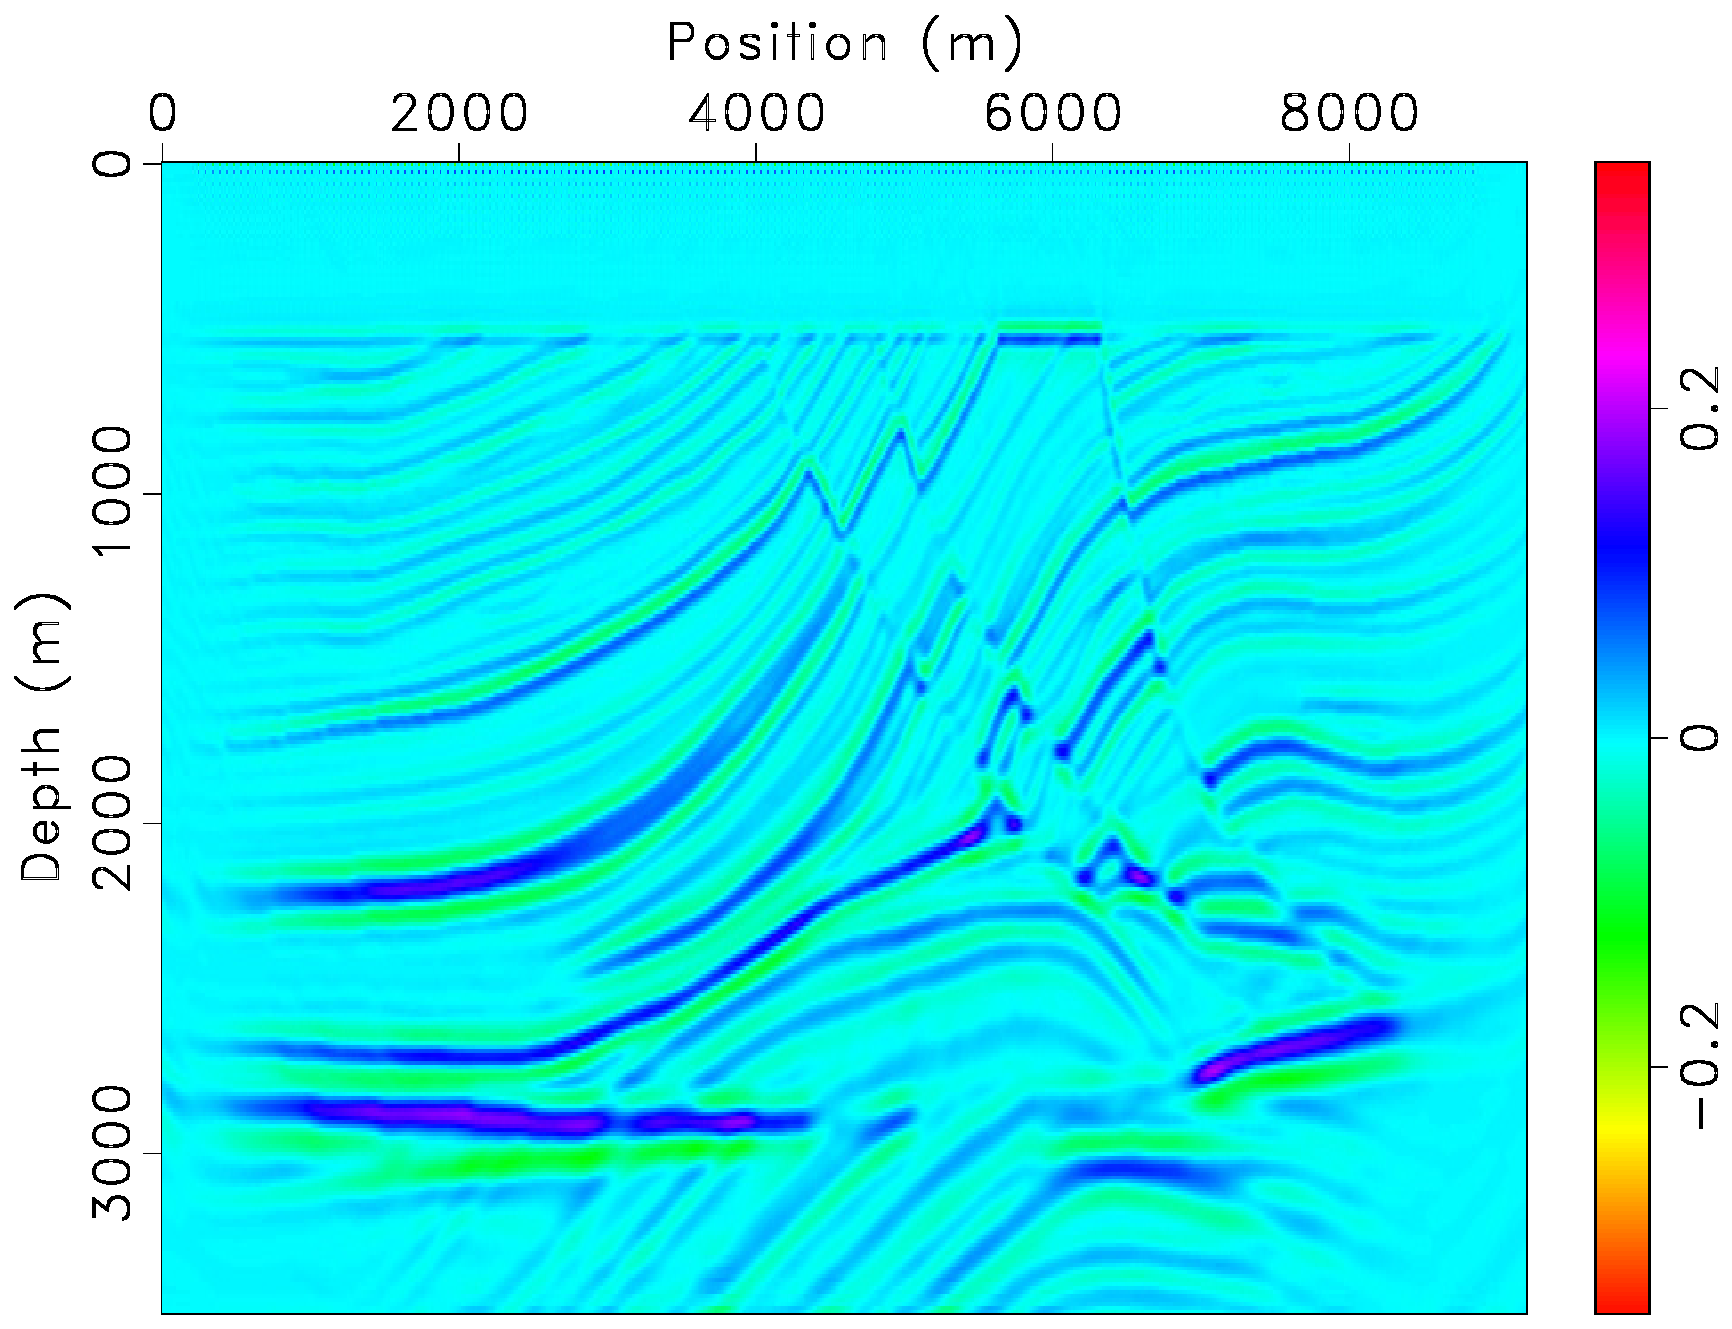
\includegraphics[height=6.8cm]{Fig/fine1bulkinvp1it0}\\
$(I_tF)^{\dagger}(I_tF)\delta \kappa$ = TAM
\end{center}
\end{frame}

\begin{frame}
\vspace{-0.5cm}
\begin{center}
%\includegraphics[height=7cm]{Fig/coarse1dbulk1}\\
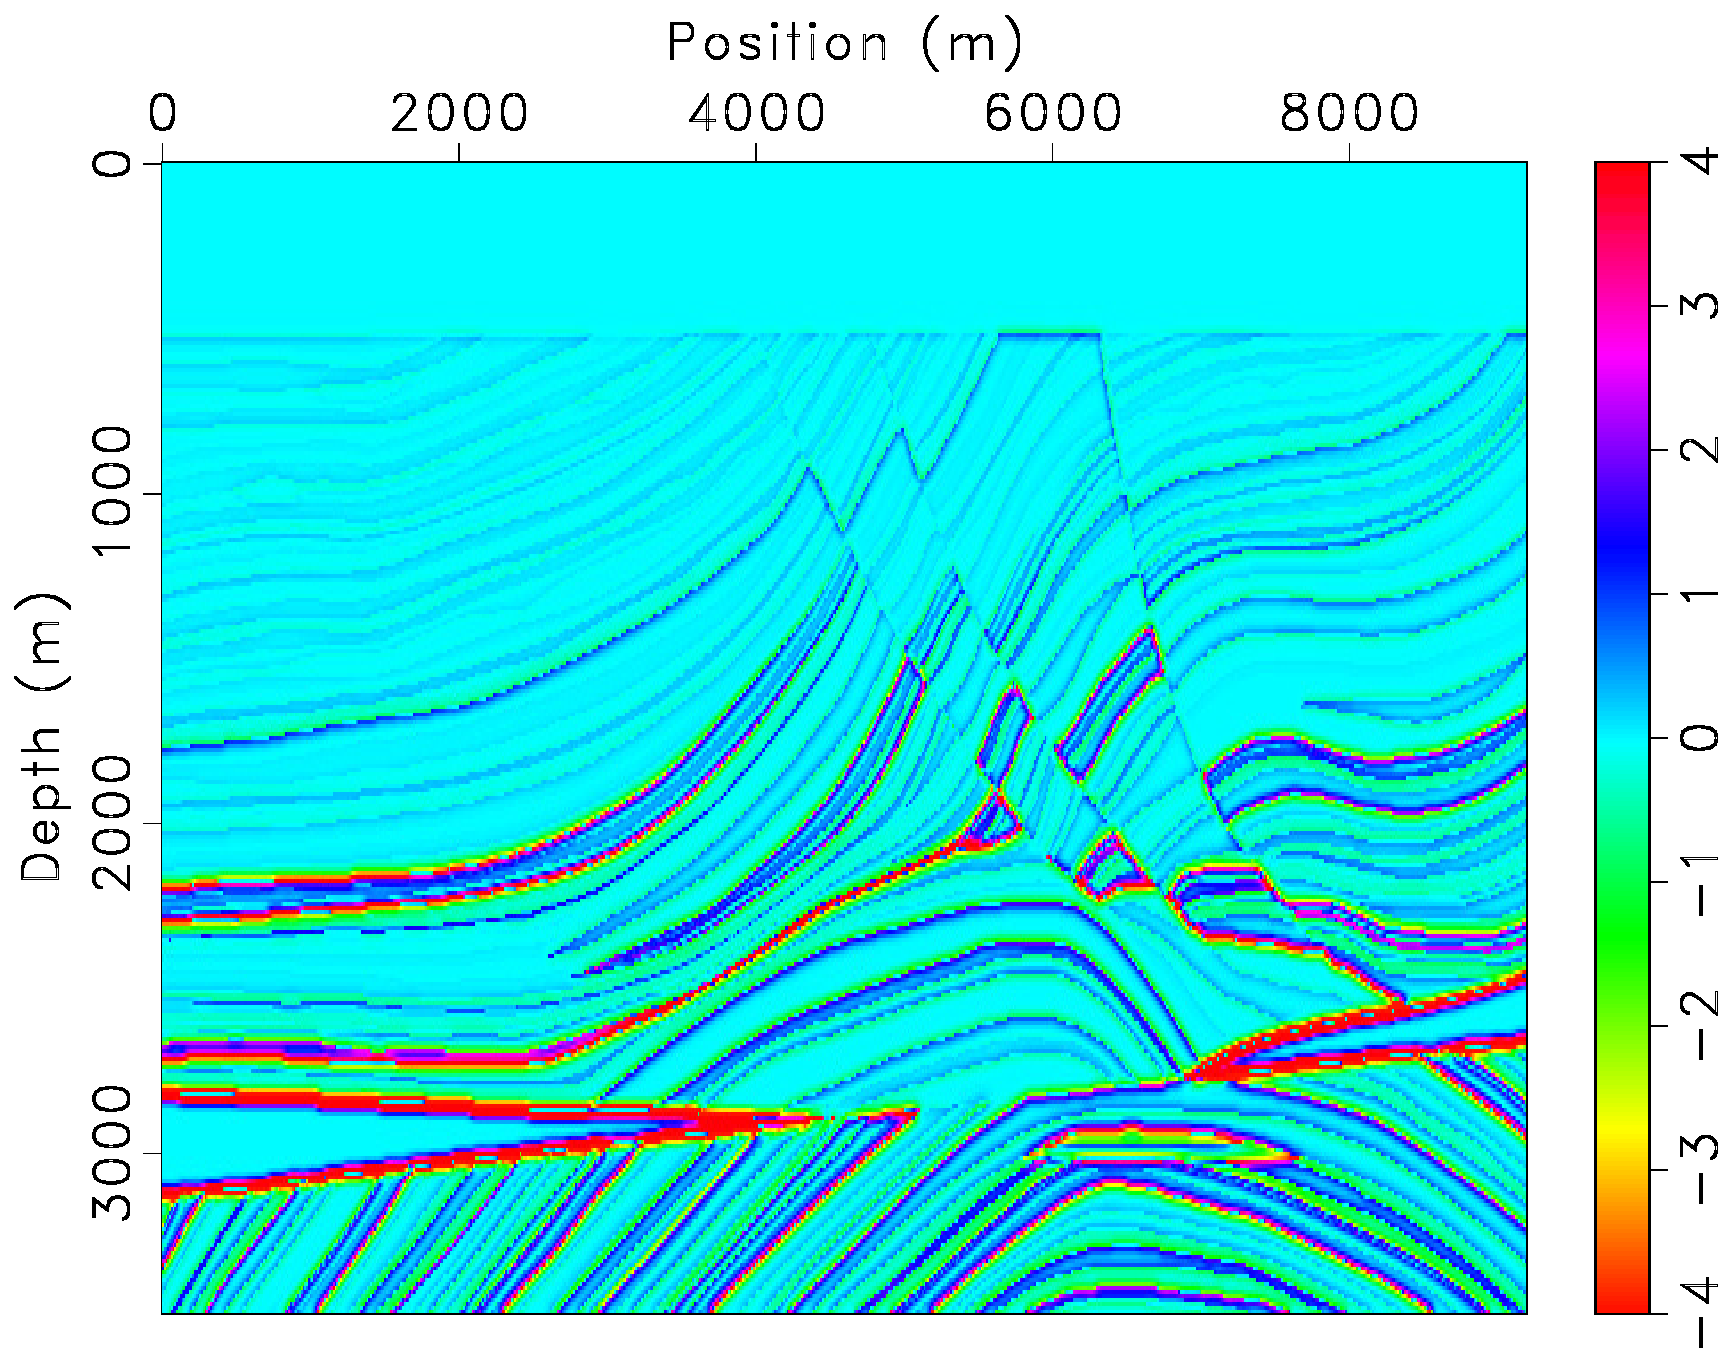
\includegraphics[height=7cm]{Fig/fine1dbulk}\\
$\delta \kappa$ = model perturbation
\end{center}
\end{frame}

\begin{frame}
Observations:
\begin{itemize}
\item reflector positions still correct
\item amplitudes, spectrum much better balanced 
\item low frequency noise absent
\item {\color{blue} not an approximate inversion - absolute amplitudes too small}
\end{itemize}

Constraints:
\begin{itemize}
\item absorbing surface data: $z_s,z_r=0$
\item DSR hypothesis: rays involved in imaging migration aperture {\em do not turn}
\end{itemize}
\end{frame}


\section{Computing TAM}

\begin{frame}
\begin{itemize}
\item Accessing $z_s,z_r$ derivatives
\item Migrating free surface data
\end{itemize}
\end{frame}

\begin{frame}
Access to $D_{z_s,r}$ via {\em shallow tow depth} hypothesis (Hou \& S. 15): $F^{\rm free}$ = free surface data with $z_s, z_r > 0$,
\[
D_{z_s}D_{z_r}F \approx \frac{1}{4 z_r z_s}F^{\rm free}
\]
Error = $O(z_s^2, z_r^2)$ = same order as FD RTM error if $z_{s,r} = O(\Delta z)$

$D_{z_s}D_{z_r}$ {\em symmetric} $\Rightarrow$
\[
(I_tF)^{\dagger} = -W_m^{-1}(I_tF)^T|f|^{-3}D_{z_s}D_{z_r} = -W_m^{-1}[D_{z_s}D_{z_r}(I_tF)]^T|f|^{-3}
\]
\[
=-\frac{1}{4 z_r z_s}W_m^{-1}(I_tF^{\rm free})^T|f|^{-3}
\]
\end{frame}


\begin{frame}
More work - similar for free surface TAM
\[
(I_tF^{\rm free})^{\dagger} =-\frac{1}{4 z_r z_s}W_m^{-1}(I_tF)^T|f|^{-3}
\]

{\bf NB:} {\em all} examples shown here actually free surface, $F \rightarrow F^{\rm free}$

TAM workflow, free surface data:
\begin{itemize}
\item filter by $|f|^{-3}$
\item absorbing surface RTM with Heaviside source pulse ($I_t$)
\item apply $W_m^{-1}$ - filter by $|k_z|$, scale
\end{itemize}

All steps except RTM - trace-by-trace filters, scaling ops $\Rightarrow$ {\color{blue} negligible expense beyond RTM}
\end{frame}

\begin{frame}
Observations:

\begin{itemize}
\item ghost construction of $(I_tF^{\rm free})^{\dagger}$ only works for tow depth $<<$ wavelength - vulnerable to depth variations, swell noise,...
\item input $D_{z_s}D_{z_r} d$ to RTM $\Leftrightarrow$ use data, source traces as Dirichlet conditions on $z=0$ (Zhang et al. 09, 11, 14,...)
\item other acquisition geometries: 
\begin{itemize}
\item 4C OBCs, shallow tow depth sources: $D_{z_r}p \propto v_z$ 
\item Geostreamer$^{\rm TM}$ - measure $v_z$
\item ...
\end{itemize}
\end{itemize}
\end{frame}


\section{TAM as Preconditioner}

\begin{frame}
Form of approx scaled inverse $(I_tF)^{\dagger} = W_m^{-1}(I_tF)^TW_d$ $\Rightarrow$ can apply
PCG (eg. Golub \& van Loan 2012) - minimizes

\[
J[\delta \kappa] = (I_t (d-F\delta \kappa))^T W_d (I_t(d-F\delta \kappa))
\]

{\bf NB:} $W_d$ plays no explicit role in step!

\begin{itemize}
\item application of {\em model-unweighted} adjoint $(I_tF)^TW_d = -\frac{1}{4 z_r z_s}(I_tF^{\rm free})^T|f|^{-3}$
\item application of $W_m^{-1}$
\item dot products, vector arithmetic
\item similar for $F^{\rm free}$
\end{itemize}
\end{frame}

\begin{frame}
\vspace{-0.62cm}
\begin{center}
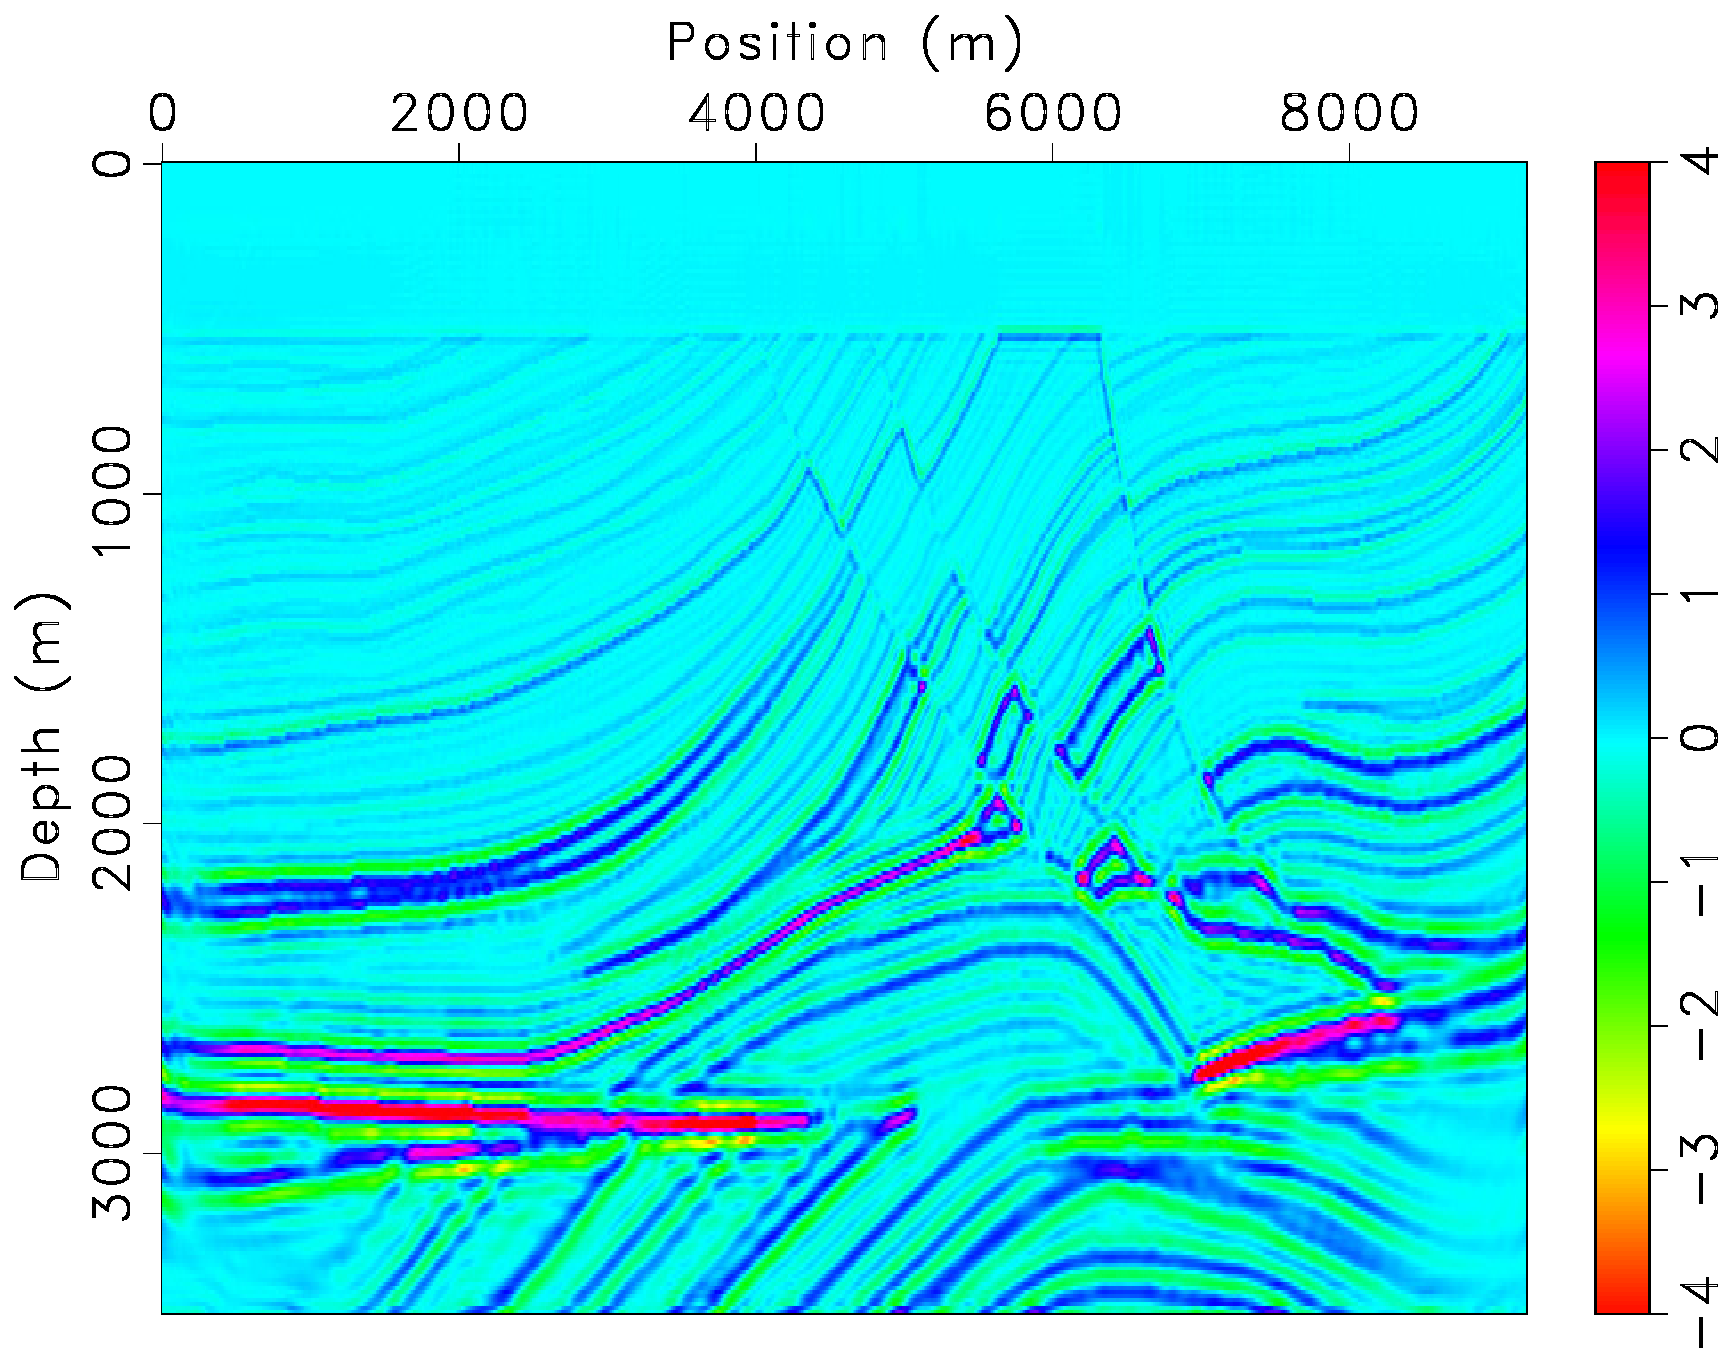
\includegraphics[height=6.8cm]{Fig/fine1bulkinvp1it20}\\
$\delta \kappa$ estimate, 20 iterations TAM-preconditioned CG
\end{center}
\end{frame}

\begin{frame}
\vspace{-0.5cm}
\begin{center}
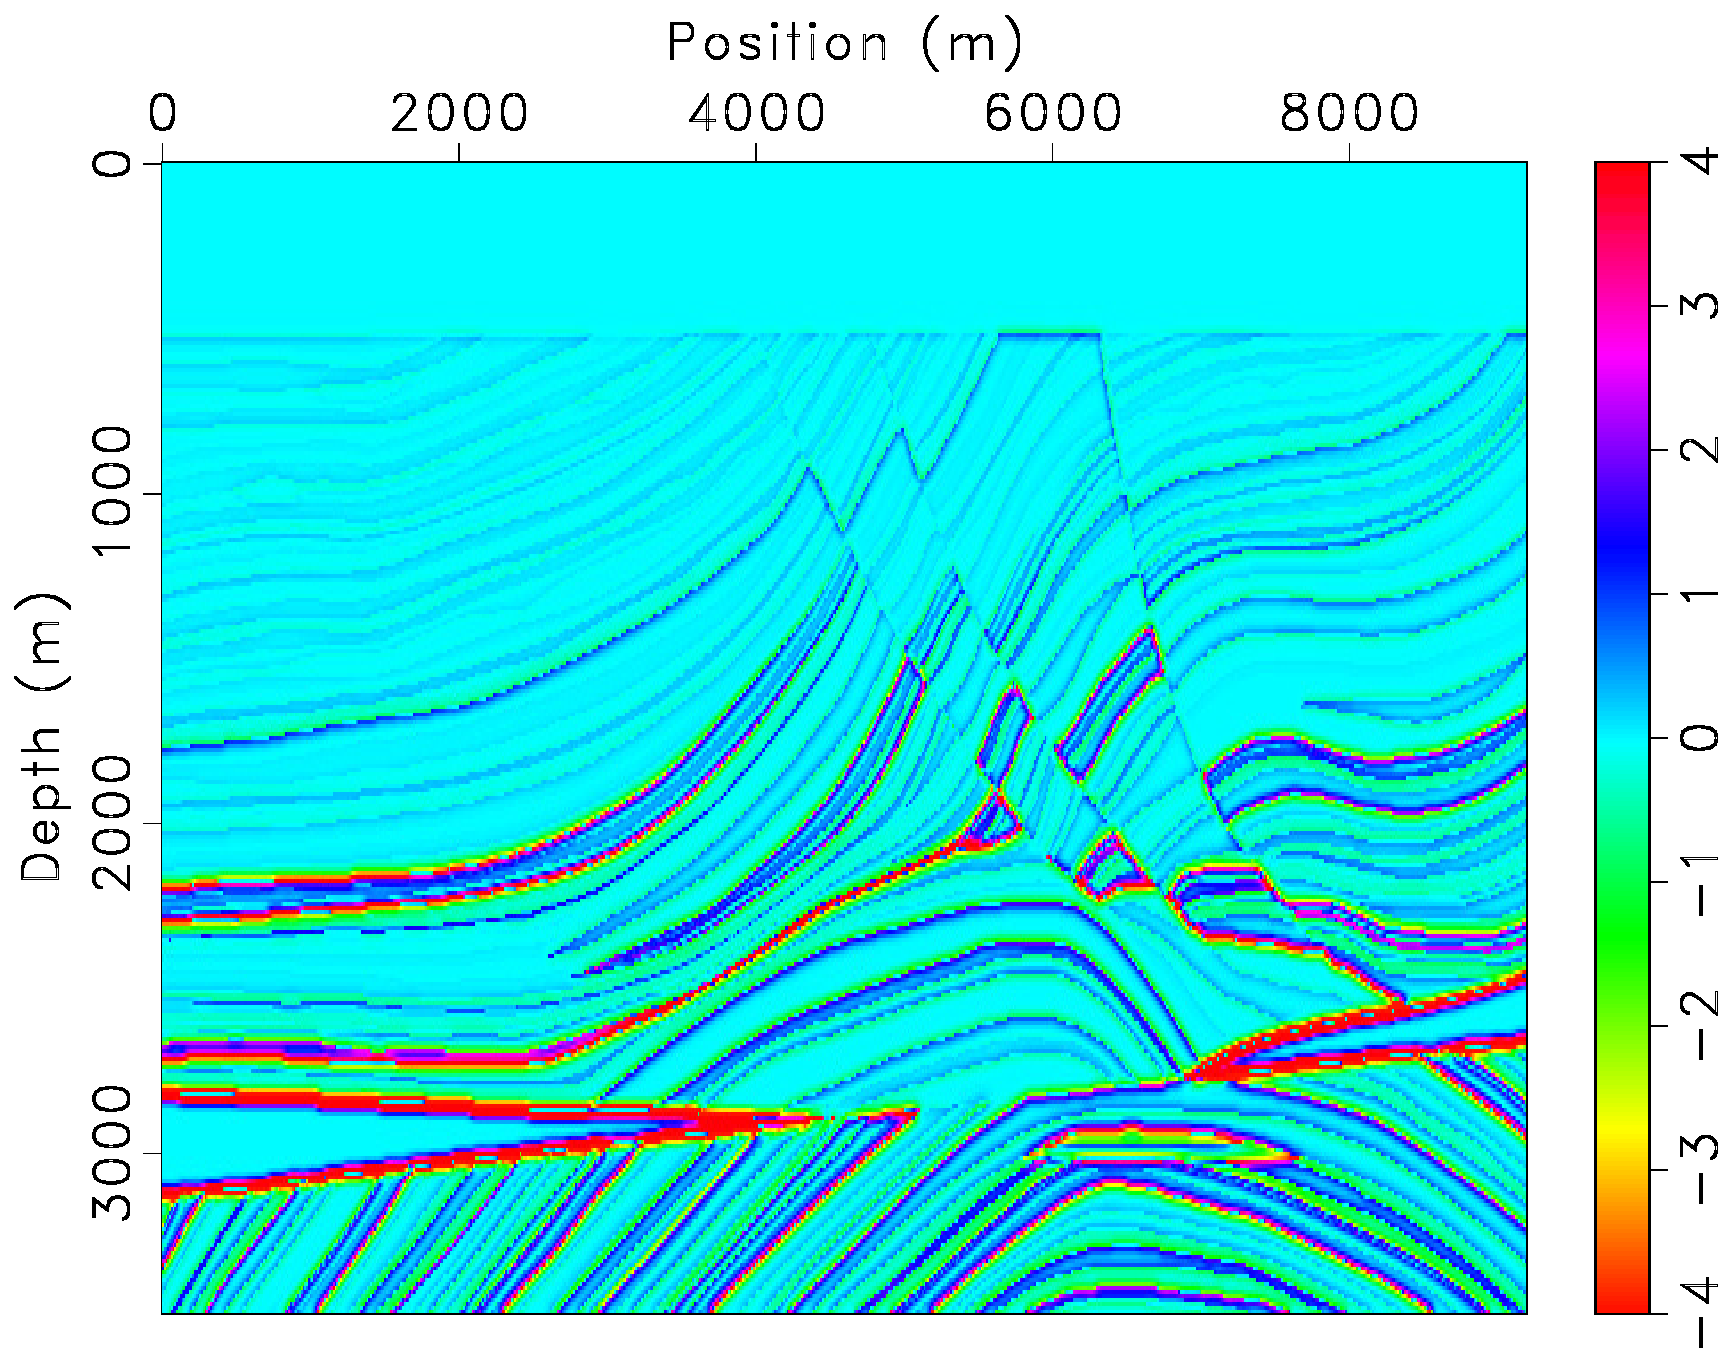
\includegraphics[height=7cm]{Fig/fine1dbulk}\\
$\delta \kappa$ = target model perturbation
\end{center}
\end{frame}

\begin{frame}
\vspace{-0.5cm}
\begin{center}
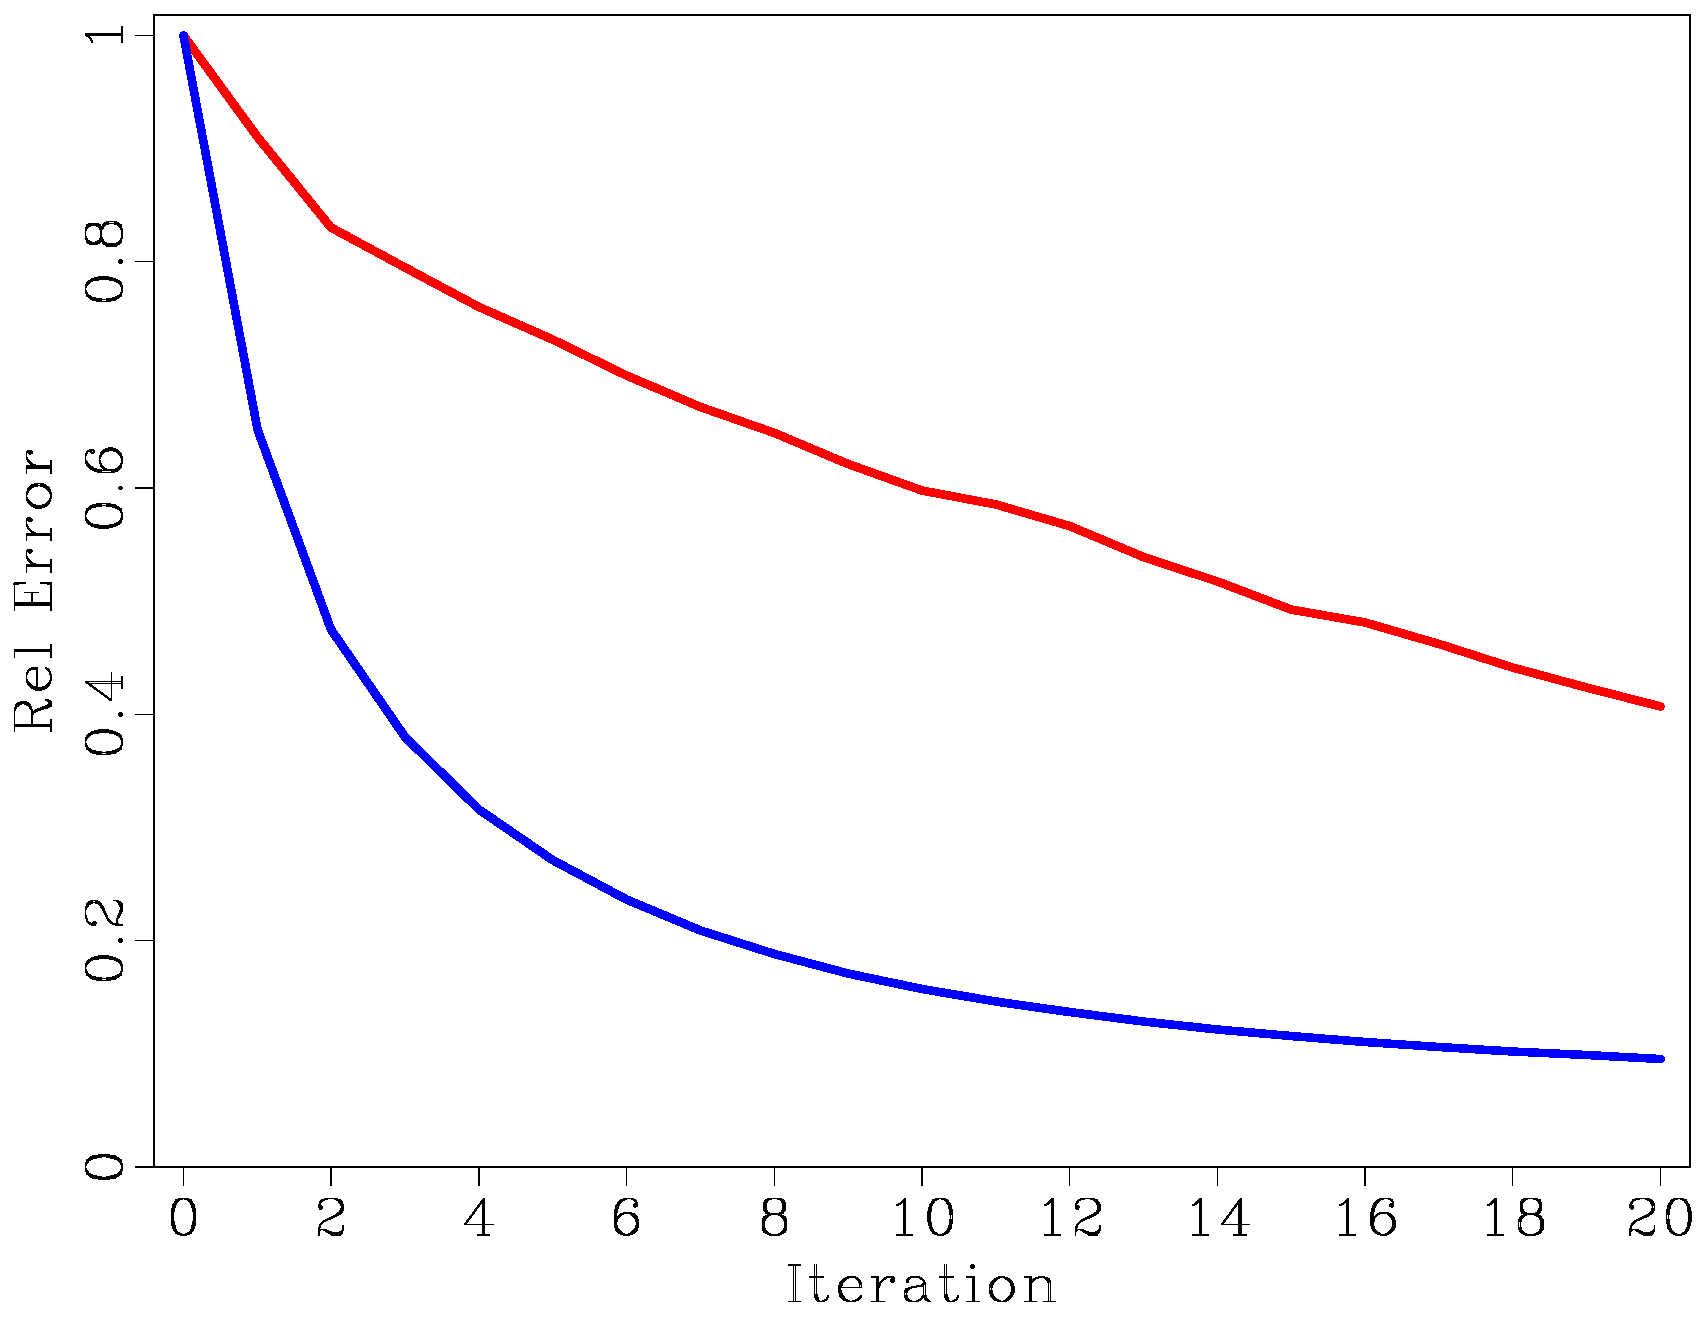
\includegraphics[height=7cm]{Fig/fine1comp}\\
Mean square error (unweighted!) vs. iteration: Red = CG, Blue = PCG
\end{center}
\end{frame}

\begin{frame}
Observations:
\begin{itemize}
\item $(I_tF)^{\dagger}$, $(I_tF^{\rm free})^{\dagger}$ not approx inverses - differs by slowly varying scale factor $< 1$
\item reason: = zero-offset section of band-limited subsurface offset approximate inverse (ten Kroode 12, Hou \& Symes 15, 17, Chauris \& Cocher 17) 
\item like $t=0$ value of band-limited impulse
\item doesn't matter - preconditioning still compresses spectrum 
\item major issue: must ensure that $W_d$ positive
\end{itemize}
\end{frame}

\begin{frame}
Positivity of $W_d$:  source, receiver slownesses have same sign,
\[
-|f|^{-2}D_{z_r}D_{z_s} = -\frac{ik_{z_s}}{f}\frac{ik_{z_r}}{f} > 0
\]

Sufficient condition (absorbing surface): sources, receivers in non-reflecting near-surface layer (``ocean'') - {\em cannot permit artificial reflectors to develop in layer during iteration}

For sources, receivers in water layer: depth-taper, $\delta \kappa = 0$ near surface in every iteration
\end{frame}

\begin{frame}
\vspace{-0.5cm}
\begin{center}
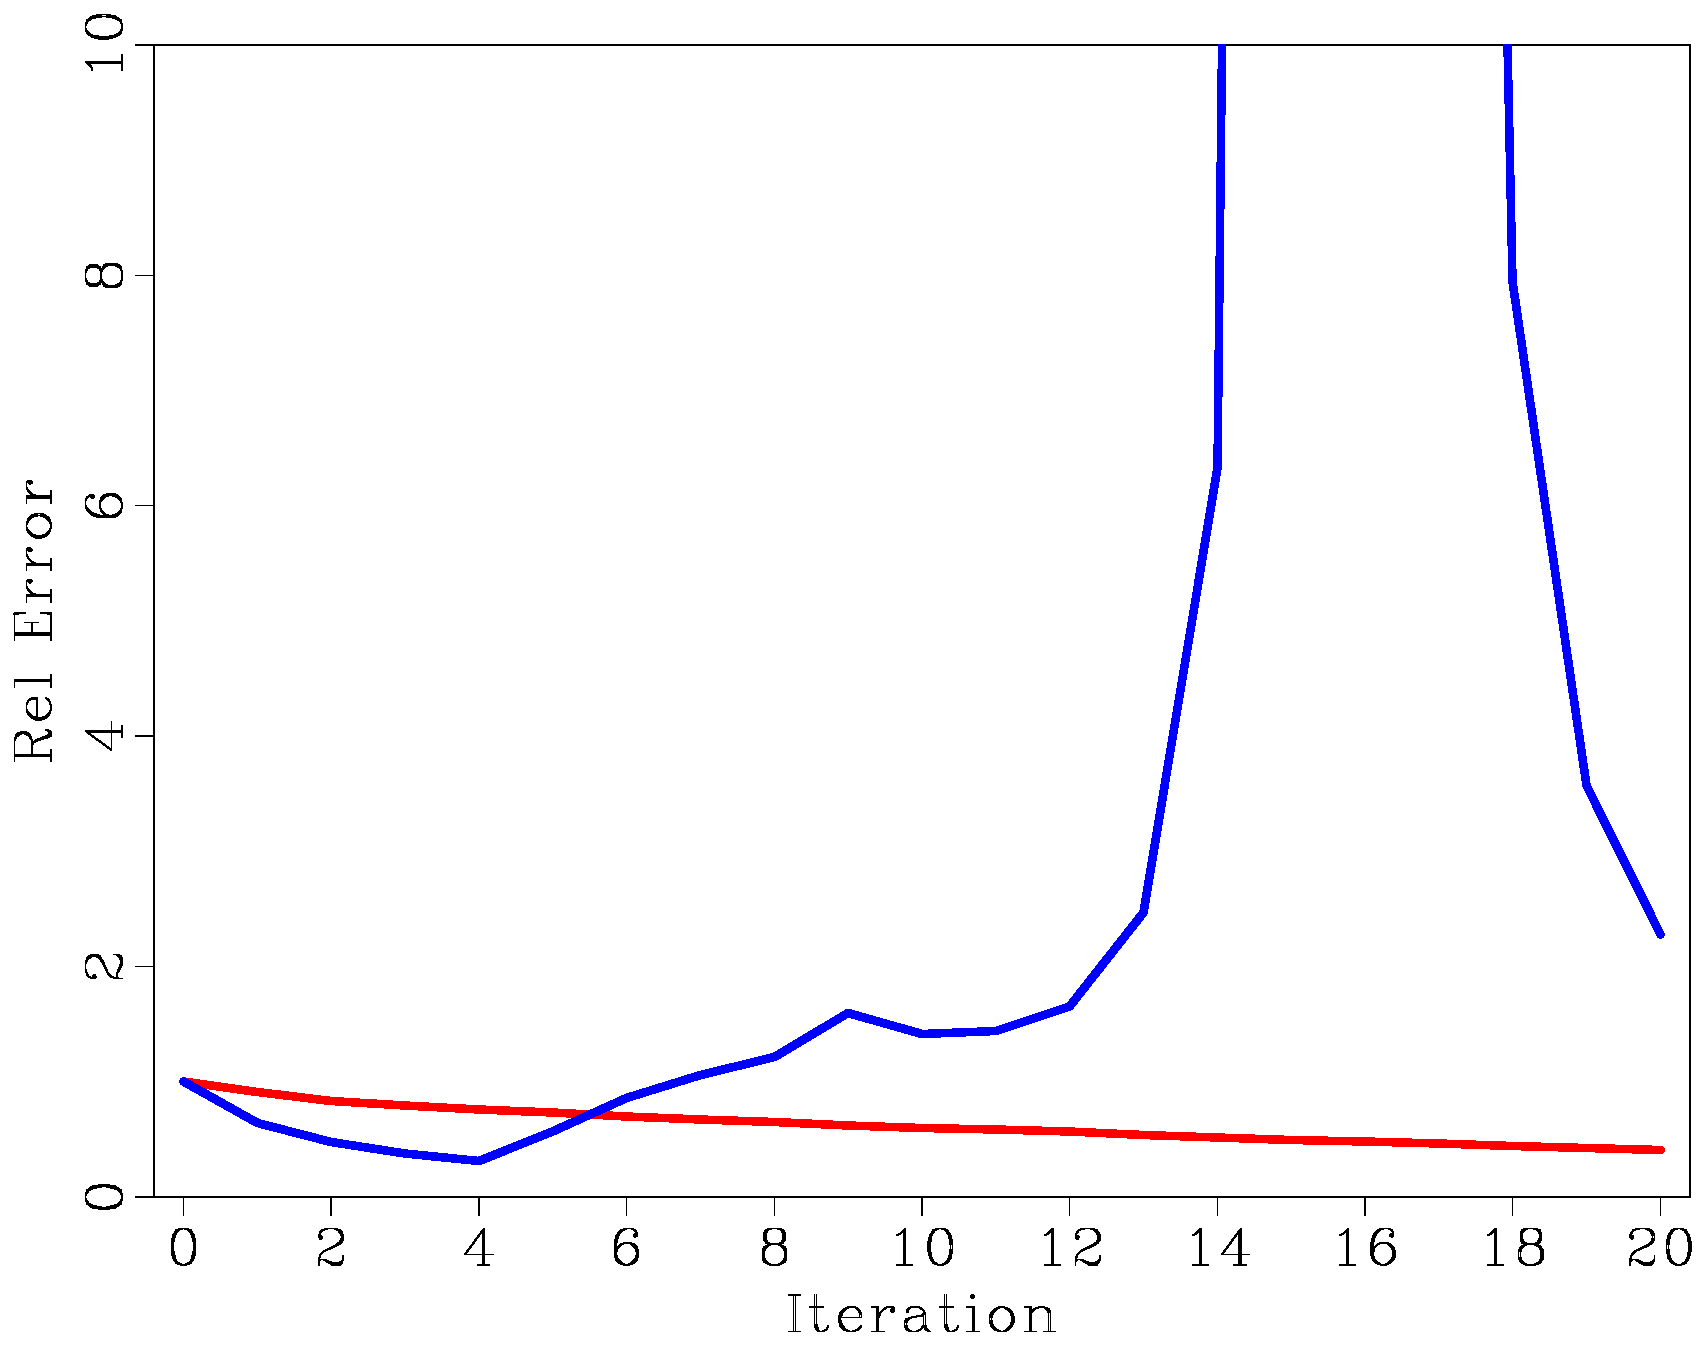
\includegraphics[height=6cm]{Fig/fine1compnt}\\
Residual curves without depth-taper on $\delta \kappa$ - Red = CG, Blue = PCG. Horizontally propagating noise $\Rightarrow$ artificial reflectors imaged in water $\Rightarrow$ non-positive data weight, leads to divergence of PCG
\end{center}
\end{frame}

\section{Summary, Prospects}

\begin{frame}
``True Amplitude'' RTM can serve as effective preconditioner for least squares migration

Reason: can be written as {\em transpose of $F$ using weighted dot products}

``Ghost trick'' for free surface TARTM $\Rightarrow$ $W_d$ implicit, uses absorbing surface RTM

Essential: $W_d > 0$: sufficient to ensure downgoing source, upcoming receiver wave fields

TARTM differs from approximate inverse by slowly varying amplitude factor - still works as preconditioner!
\end{frame}

\begin{frame}\frametitle{Acknowledgements}
\begin{itemize}
\item A. ten Kroode, J. Hou
\item Shell 
\item sponsors of The Rice Inversion Project
\item Texas Advanced Computing Center, U. of Texas, Austin
\end{itemize}
\end{frame}

\end{document}